\graphicspath{{Chapters/CrossSection/Figures/}}
\chapter{Observed Events and \CX\ Measurement}
\label{chap:CrossSection}

\section{Observed Events}

The observed and expected event yields after applying the \ZZ\ and \ZZs\ selections are shown
in~\tab{obs-expected-events-seven} for the 7~\tev\ analysis and
in~\tab{obs-expected-events-eight} for the 8~\tev\ analysis. 
A total
of~\ZZSevenTeVNObsZZLLLL\ events
are observed in \LumiPassGRLTwentyEleven~\ifb\ of 7~\tev\ data for the \ZZ\ selection, and a total of~\ZZSevenTeVNObsZZLLLL\ events for the \ZZs\ selection. In the 8~\tev\ data, which corresponds to an integrated luminosity of
\LumiPassGRLTwentyTwelve~\ifb, \ZZEightTeVNObsZZLLLL\ events are observed for
the \ZZ\ selection.
%and \ZZEightTeVNObsZZsLLLL\ for the \ZZs\ selection.

%% Expected and observed events, 7 TeV
\begin{table}
\centering
\small
  \begin{tabular}{lcccc}
    \hline\hline
     7~\tev, \ZZ             & \eeee & \mmmm & \eemm & \llll \\
     \hline
Observed & 16 & 23 & 27 & 66 \\
% Systematic is reco+gen_diff+pdf+scale
Exp. Signal &   10.3 $\pm$ 0.1 $\pm$ 1.0 &  16.5 $\pm$ 0.2 $\pm$ 0.9 &  26.7 $\pm$ 0.2 $\pm$ 1.7 &  53.4 $\pm$ 0.3 $\pm$ 3.2 \\
Exp. Bg. & 
    \ZZSevenTeVTotalBgEstZZEEEE &
    \ZZSevenTeVTotalBgEstZZMMMM &
    \ZZSevenTeVTotalBgEstZZEEMM &
    \ZZSevenTeVTotalBgEstZZLLLL \\
\hline\hline
    \\
    \hline\hline
     7~\tev, \ZZs             & \eeee & \mmmm & \eemm & \llll \\
     \hline
Observed & 21 & 30 & 33 & 84 \\
% Systematic is reco+gen_diff+pdf+scale
Exp. Signal &  12.3 $\pm$ 0.2 $\pm$ 1.2 &  20.5 $\pm$ 0.2 $\pm$ 1.1 &  31.6 $\pm$ 0.3 $\pm$ 2.0 &  64.4 $\pm$ 0.4 $\pm$ 4.0 \\
Exp. Bg. & 
    \ZZSevenTeVTotalBgEstZZsEEEE &
    \ZZSevenTeVTotalBgEstZZsMMMM &
    \ZZSevenTeVTotalBgEstZZsEEMM &
    \ZZSevenTeVTotalBgEstZZsLLLL \\
    \hline\hline
  \end{tabular}

      \caption[Expected and observed events in \LumiPassGRLTwentyEleven~\ifb\ of
      7~\tev\ data.]
      {Number of observed events passing the \ZZ\ (top table) and \ZZs\
      (bottom table) selections in \LumiPassGRLTwentyEleven~\ifb\ of 7~\tev\
      data, as well as the expected number of signal events (Exp.~Signal) and
      the expected background (Exp.~Bg.).  The expected background is the sum of
      the data driven estimate for the reducible background and the \mc\
      estimated for the irreducible background. The first uncertainty is statistical, while the second is
      systematic; uncertainties on the integrated luminosity
      (\LumiUncTwentyEleven) are not included.  }
\label{table:obs-expected-events-seven}
\end{table}

%% Expected and observed events, 8 TeV
\begin{table}
\centering
\small
  \begin{tabular}{lcccc}
    \hline\hline
     8~\tev, \ZZ             & \eeee & \mmmm & \eemm & \llll \\
     \hline
Observed & \ZZEightTeVNObsZZEEEE & \ZZEightTeVNObsZZMMMM & \ZZEightTeVNObsZZEEMM & \ZZEightTeVNObsZZLLLL \\
Exp. Signal &   
    \ZZEightTeVNExpZZEEEEOneDp~\errSym{\ZZEightTeVNExpStatZZEEEEOneDp}~\errSym{\ZZEightTeVNExpStatZZEEEEOneDp} & 
    \ZZEightTeVNExpZZMMMMOneDp~\errSym{\ZZEightTeVNExpStatZZMMMMOneDp}~\errSym{\ZZEightTeVNExpStatZZMMMMOneDp} & 
    \ZZEightTeVNExpZZEEMMOneDp~\errSym{\ZZEightTeVNExpStatZZEEMMOneDp}~\errSym{\ZZEightTeVNExpStatZZEEMMOneDp} & 
    \ZZEightTeVNExpZZLLLLOneDp~\errSym{\ZZEightTeVNExpStatZZLLLLOneDp}~\errSym{\ZZEightTeVNExpStatZZLLLLOneDp} \\
Exp. Bg. & 
    \ZZEightTeVTotalBgEstZZEEEE &
    \ZZEightTeVTotalBgEstZZMMMM &
    \ZZEightTeVTotalBgEstZZEEMM &
    \ZZEightTeVTotalBgEstZZLLLL \\
\hline\hline
%    \\
%    \hline\hline
%     8~\tev, \ZZs             & \eeee & \mmmm & \eemm & \llll \\
%     \hline
%Observed & \ZZEightTeVNObsZZEEEE & \ZZEightTeVNObsZZMMMM & \ZZEightTeVNObsZZEEMM & \ZZEightTeVNObsZZLLLL \\
%Exp. Signal &   
%    \ZZEightTeVNExpZZsEEEE~\errSym{\ZZEightTeVNExpStatZZsEEEE}~\errSym{\ZZEightTeVNExpStatZZsEEEE} & 
%    \ZZEightTeVNExpZZsMMMM~\errSym{\ZZEightTeVNExpStatZZsMMMM}~\errSym{\ZZEightTeVNExpStatZZsMMMM} & 
%    \ZZEightTeVNExpZZsEEMM~\errSym{\ZZEightTeVNExpStatZZsEEMM}~\errSym{\ZZEightTeVNExpStatZZsEEMM} & 
%    \ZZEightTeVNExpZZsLLLL~\errSym{\ZZEightTeVNExpStatZZsLLLL}~\errSym{\ZZEightTeVNExpStatZZsLLLL} \\
%Exp. Bg. & 
%    \ZZEightTeVNBgZZsEEEE~\errSym{\ZZEightTeVNBgStatZZsEEEE}~\errSym{\ZZEightTeVNBgStatZZsEEEE} & 
%    \ZZEightTeVNBgZZsMMMM~\errSym{\ZZEightTeVNBgStatZZsMMMM}~\errSym{\ZZEightTeVNBgStatZZsMMMM} & 
%    \ZZEightTeVNBgZZsEEMM~\errSym{\ZZEightTeVNBgStatZZsEEMM}~\errSym{\ZZEightTeVNBgStatZZsEEMM} & 
%    \ZZEightTeVNBgZZsLLLL~\errSym{\ZZEightTeVNBgStatZZsLLLL}~\errSym{\ZZEightTeVNBgStatZZsLLLL} \\
%    \hline\hline
  \end{tabular}

      \caption[Expected and observed events in \LumiPassGRLTwentyTwelve~\ifb\ of
      8~\tev\ data.]
      {Number of observed events passing the \ZZllll\ (top table) and \ZZsllll\
      (bottom table) selections in \LumiPassGRLTwentyTwelve~\ifb\ of 8~\tev\
      data, as well as the expected number of signal events (Exp.~Signal) and
      the expected background (Exp.~Bg.).  The expected background is the sum of
      the data driven estimate for the reducible background and the \mc\
      estimated for the irreducible background. The first uncertainty is statistical, while the second is
      systematic; uncertainties on the integrated luminosity
      (\LumiUncTwentyTwelve) are not included.  }
    \label{table:obs-expected-events-eight}
\end{table}

\section{Kinematic Distributions}

\figs{zzdists-Zmass2D-seven}{zzdists-Zmass2D-eight} show the mass of the
subleading \leppair\ versus the mass of the leading \leppair\ for the 7~\tev\
and the 8~\tev\ analyses respectively. In both cases the solid red box
represents the region defined by the mass requirements of the \ZZ\ selection and
the dashed blue box the region defined by those of the \ZZs\ selection. The
events are seen to cluster in the regions where both masses are near \mZ, in
agreement with the \mc\ prediction for the signal (shown as pink boxes, with the
size of the box proportional to the number of expected events).

\fig{zzdists-dr-ptz-seven} shows the correlation between the transverse momentum
of the \leppair s and the opening-angle between the leptons forming the pair in
the 7~\tev\ data. It is observed that for higher transverse momentum \dilep\
pairs the opening-angle tends to be smaller, in good agreement with the \mc\
predictions. 

\figs{zzdists-Zmass-seven}{zzdists-Zmass-eight} show the \dilep\ invariant mass
distributions for the leading and subleading \leppair\ for the 7~\tev\ and
8~\tev\ analyses. ~\fig{zzdists-ZZ-seven} shows the
transverse momentum $\pT^{\ZZ}$ and invariant mass $m^{\ZZ}$ of the four-lepton
system, the transverse momentum of the leading \dilep\ pair $\pt^{Z1}$, and the
transverse momentum of the subleading \dilep\ pair $\pt^{Z2}$, for events
passing the \ZZ\ selection for the 7~\tev\ analysis; \fig{zzdists-ZZ-eight}
shows equivalent figure for the 8~\tev\ analysis.
\fig{zzdists-ZZs-seven} shows the corresponding
distributions for the \ZZs\ selection for the 7~\tev\ analysis. In each case the prediction from \mc\ for
the \ZZ\ signal is shown as a pink histogram and the prediction for the
background
is shown as a light blue histogram. The shapes of the distributions observed in
data are consistent with the predictions.

%~\fig{zzdists-mindr-mzz-seven} shows the minimum 

% 2D plot, 7 TeV
% Use PDF figure as text alignment is off in eps
 \begin{figure}[htbp]
 \begin{center}
  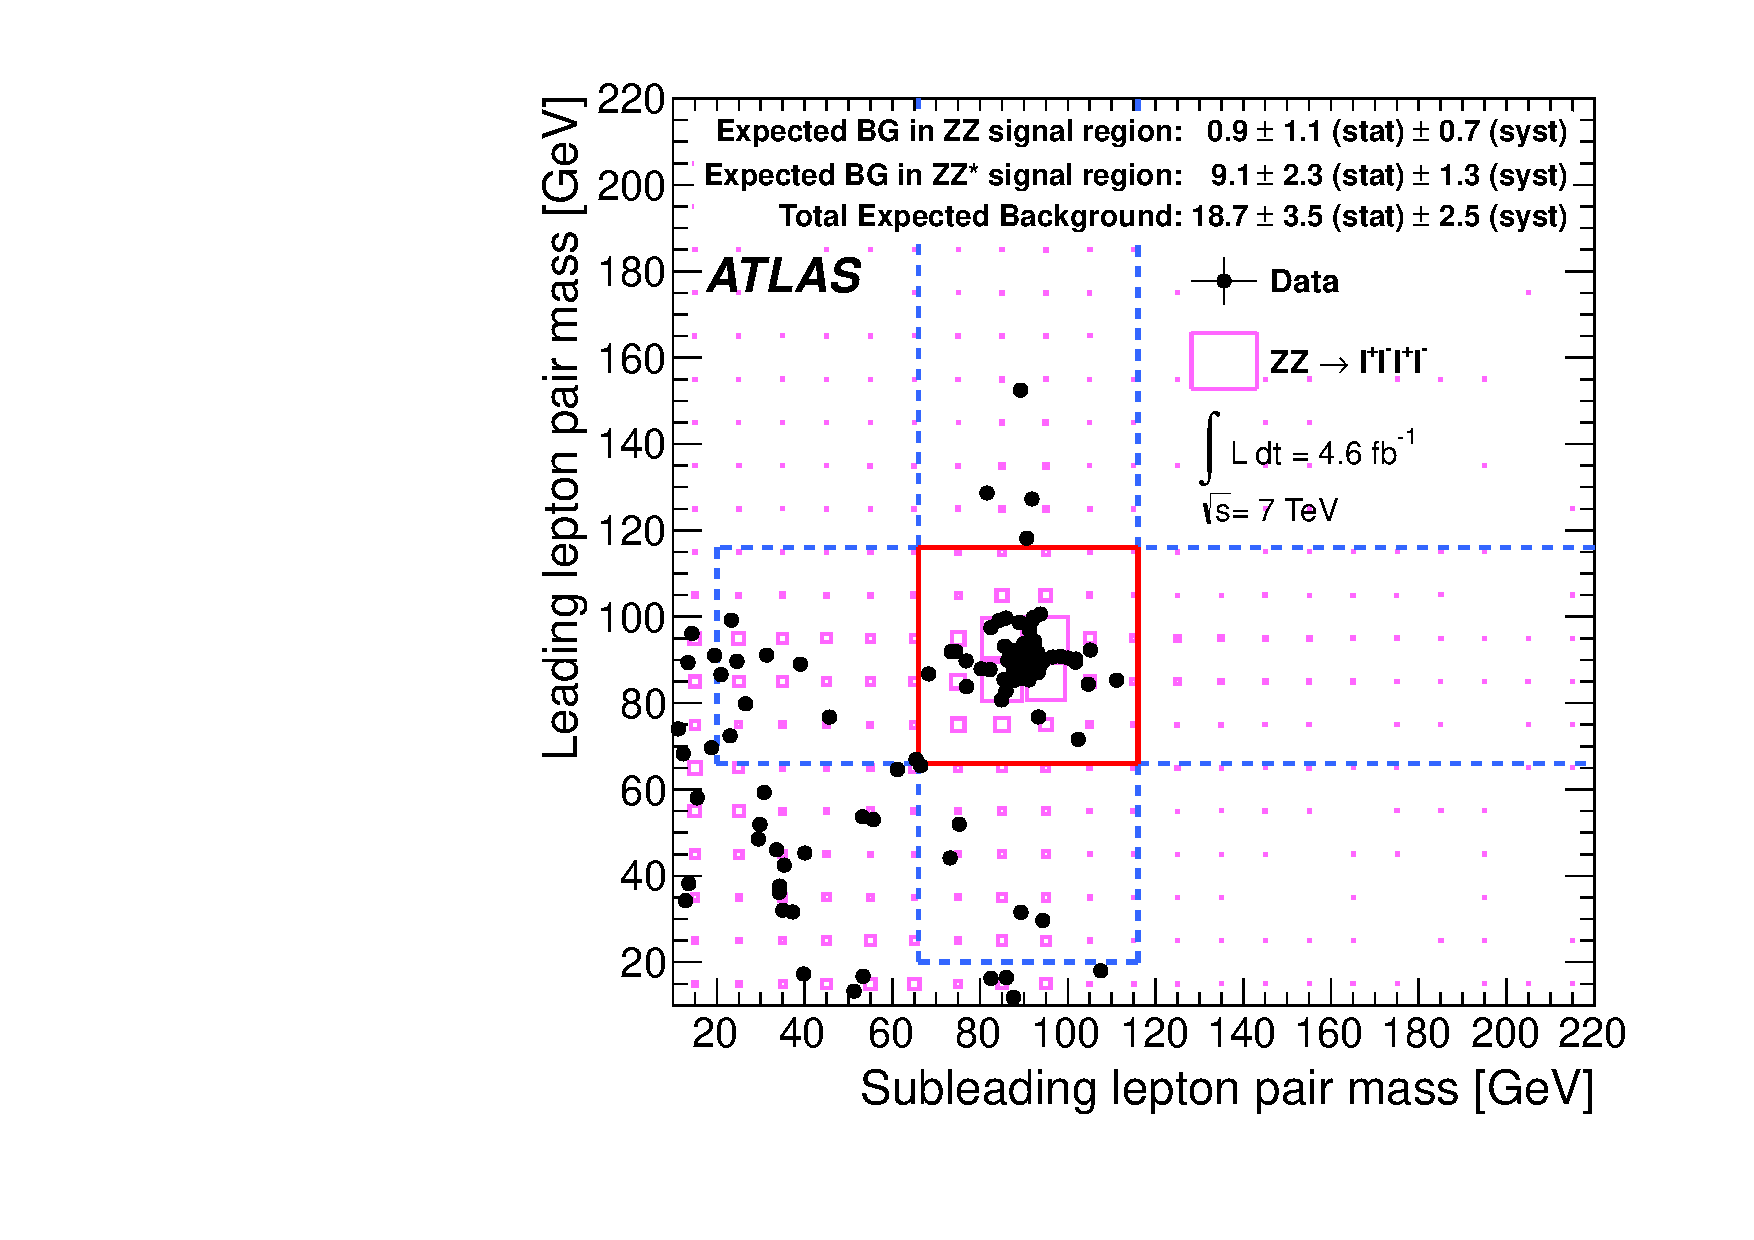
\includegraphics[width=0.7\textwidth]{7TeV/h_mz1_mz2.pdf}\hfill
  \caption[Mass of the leading \leppair\ versus the mass of the
  sub-leading \leppair\ for candidate events in 7~\tev\ data, after applying all of the selection
  requirements apart from the \dilepton\ mass requirements .]
  {\small Mass of the leading \leppair\ versus the mass of the
  sub-leading \leppair\ for candidate events in 7~\tev\ data after
  applying all of the selection
  requirements apart from the \dilepton\ mass requirements.
  The events observed in the data are shown as solid circles and the \ZZsllll\
  signal prediction from simulation as boxes,
  with the size of each box is proportional to the number of events in each bin.  
  The region enclosed by the solid (dashed) lines indicates the signal region defined by the
  \dilepton\ mass requirements for \ZZ\ (\ZZs) events.
  %The background estimate is described in section 5.1.
   }
    \label{fig:zzdists-Zmass2D-seven}
 \end{center}
 \end{figure}

% 2D plot, 8 TeV
% Use PDF figure as text alignment is off in eps
 \begin{figure}[htbp]
 \begin{center}
  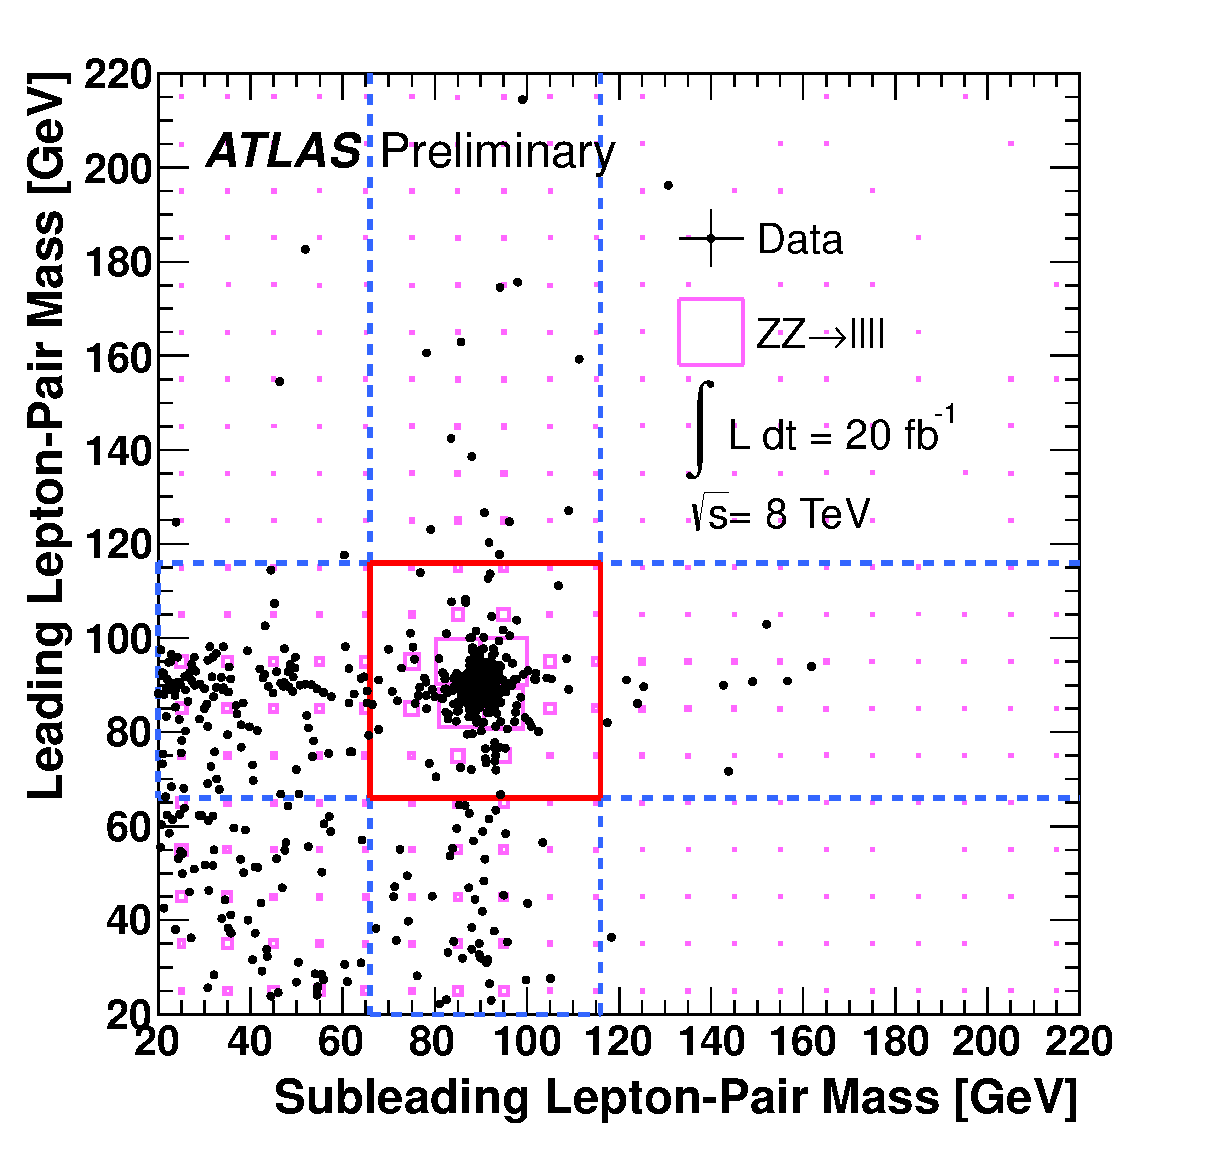
\includegraphics[width=0.7\textwidth]{8TeV/h_mz1_mz2}\hfill
  \caption[Mass of the leading \leppair\ versus the mass of the
  sub-leading \leppair\ for candidate events in 8~\tev\ data, after applying all of the selection
  requirements apart from the \dilepton\ mass requirements.]
  {\small Mass of the leading \leppair\ versus the mass of the
  sub-leading \leppair for candidate events in 8~\tev\ data after
  applying all of the selection
  requirements apart from the \dilepton\ mass requirements.
  The events observed in the data are shown as solid circles and the \ZZsllll\
  signal prediction from simulation as boxes, with 
  the size of each box is proportional to the number of events in each bin.  
  The region enclosed by the solid (dashed) lines indicates the signal region defined by the
  \dilepton\ mass requirements for \ZZ\ (\ZZs) events.
  %The background estimate is described in section 5.1.
   }
    \label{fig:zzdists-Zmass2D-eight}
 \end{center}
 \end{figure}

% pT_Z vs dR 7 TeV
 \begin{figure}[htbp]
 \begin{center}
  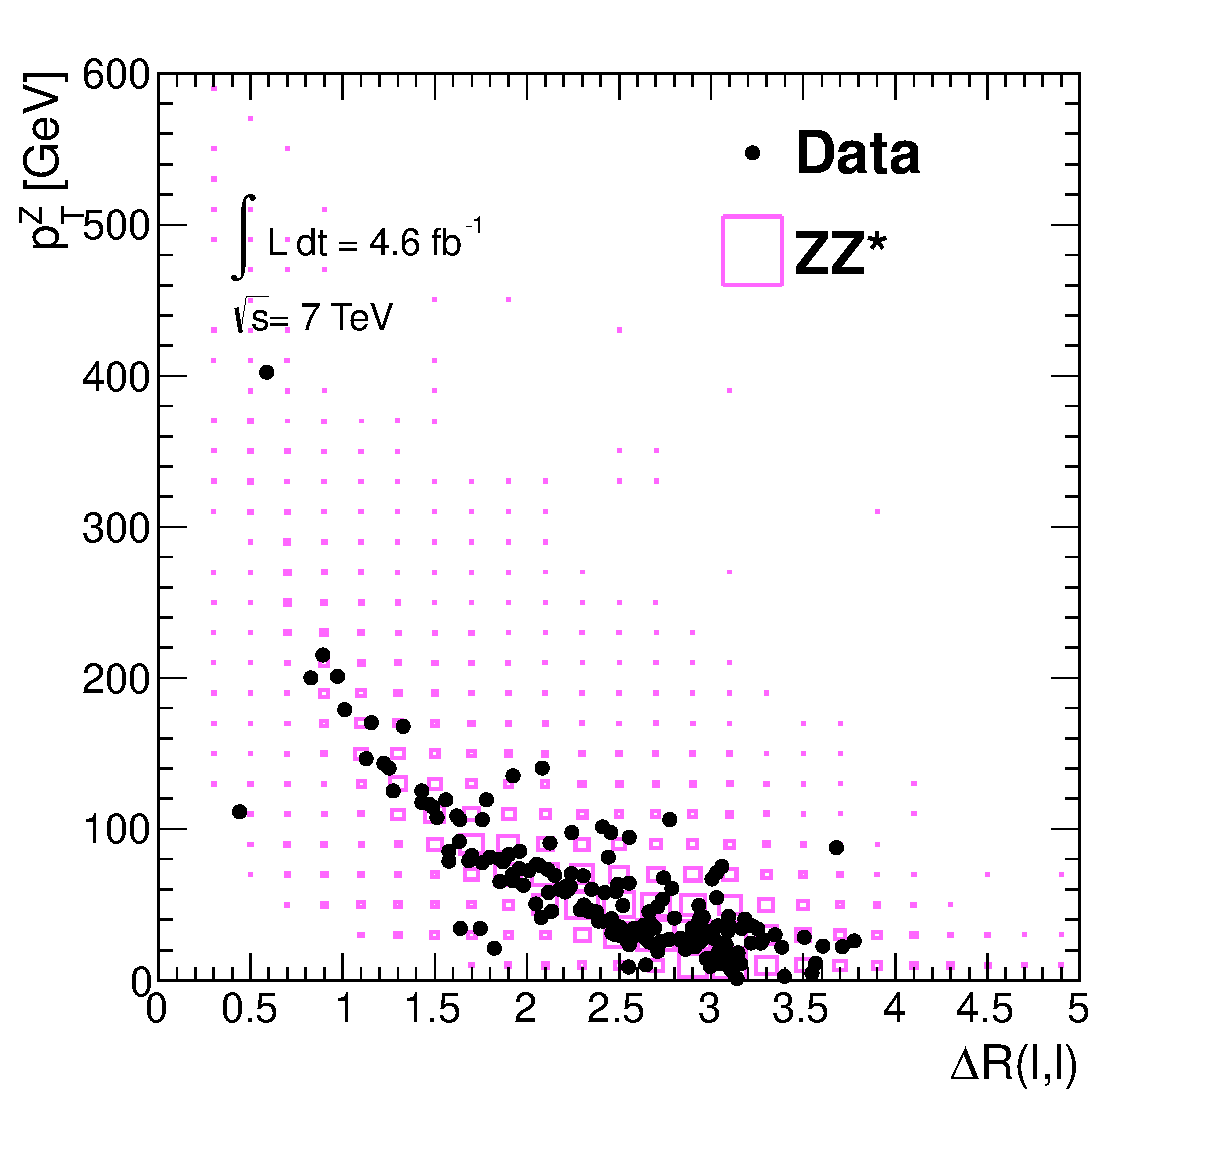
\includegraphics[width=0.7\textwidth]{7TeV/h_dr_ptz}\hfill
  \caption[Transverse momentum of \leppair s versus the opening angle between the leptons
    forming the pair, for events passing the \ZZs\ selection in 7~\tev\ data.]
    {\small Transverse momentum of  \leppair s versus the opening angle between the leptons
    forming the pair, for events passing the \ZZs\ selection in 7~\tev\ data (two
    entries per event).}
 \label{fig:zzdists-dr-ptz-seven}
 \end{center}
 \end{figure}

% m_ZZ vs min(dR) 7 TeV
% !! Not sure what this plot tells us - not much I suspect.
% \begin{figure}[htbp]
% \begin{center}
%  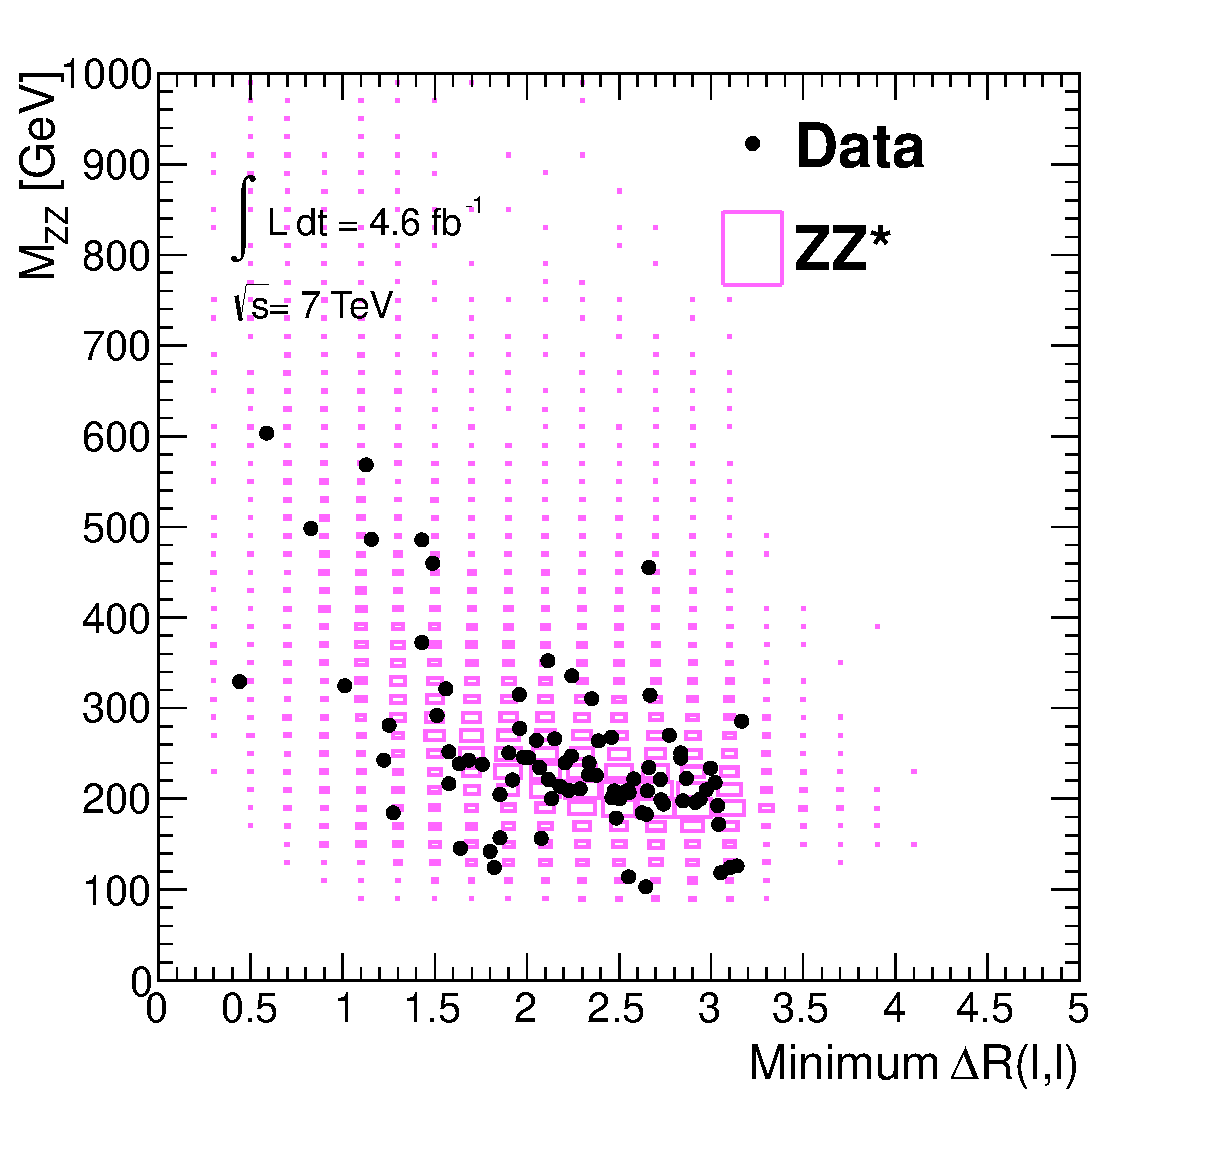
\includegraphics[width=0.7\textwidth]{7TeV/h_mindr_mzz}\hfill
%  \caption[The invariant mass of the four lepton system \mZZp\ versus the
%    minimum \deltaR\ between any pair of leptons in the event for events passing
%    the \ZZs\ selection in 7~\tev\ data.]
%    {\small The invariant mass of the four lepton system \mZZp\ versus the
%    minimum \deltaR\ between any pair of leptons in the event for events passing
%    the \ZZs\ selection in 7~\tev\ data.
%    The events observed in the data are shown as black dots and the signal prediction as boxes.}
% \label{fig:zzdists-mindr-mzz-seven}
% \end{center}
% \end{figure}

% 7 TeV, Z1_m, Z2_m, m_Z>7GeV
\begin{figure}[htbp]
    \begin{center}
     \subfigure[]{
     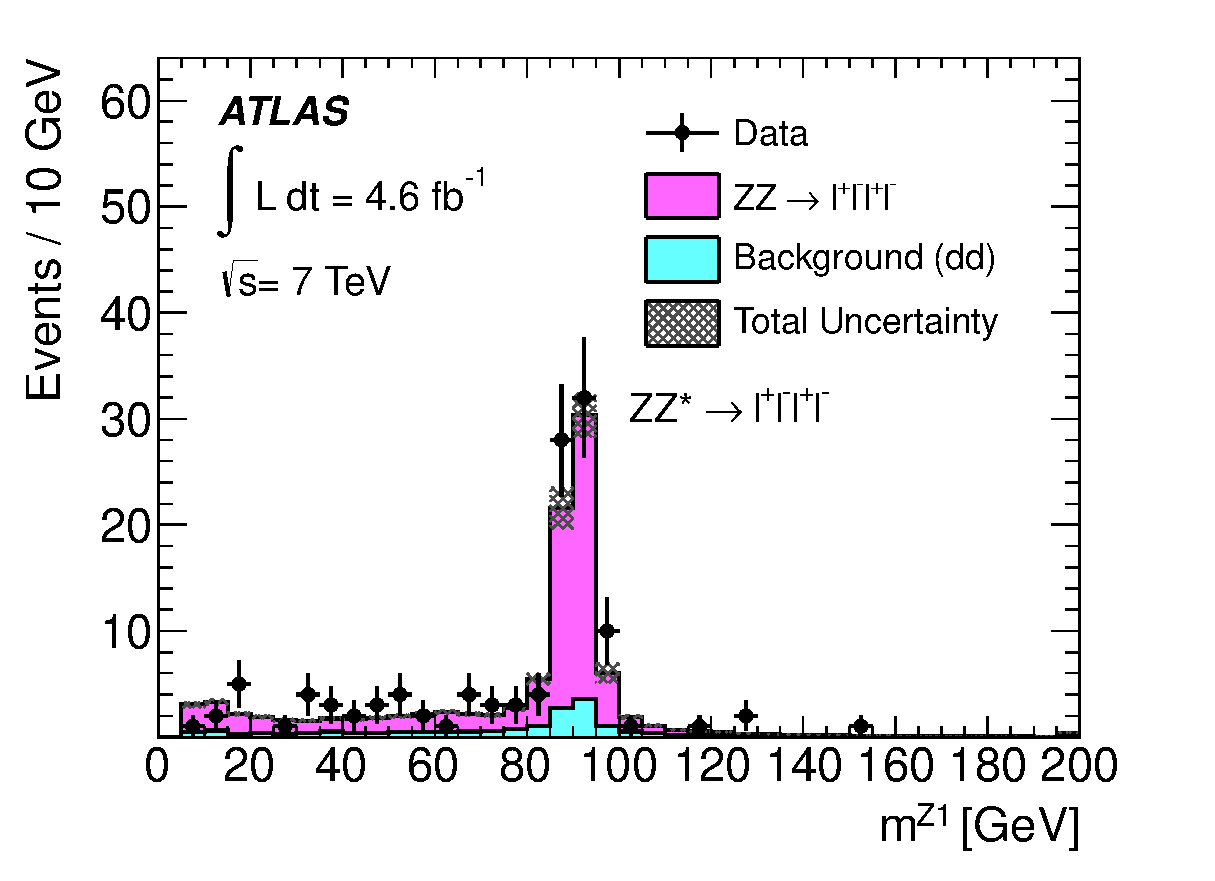
\includegraphics[width=0.47\textwidth]{7TeV/h_4l_ZZs_Z1_m}
     }
     \subfigure[]{
     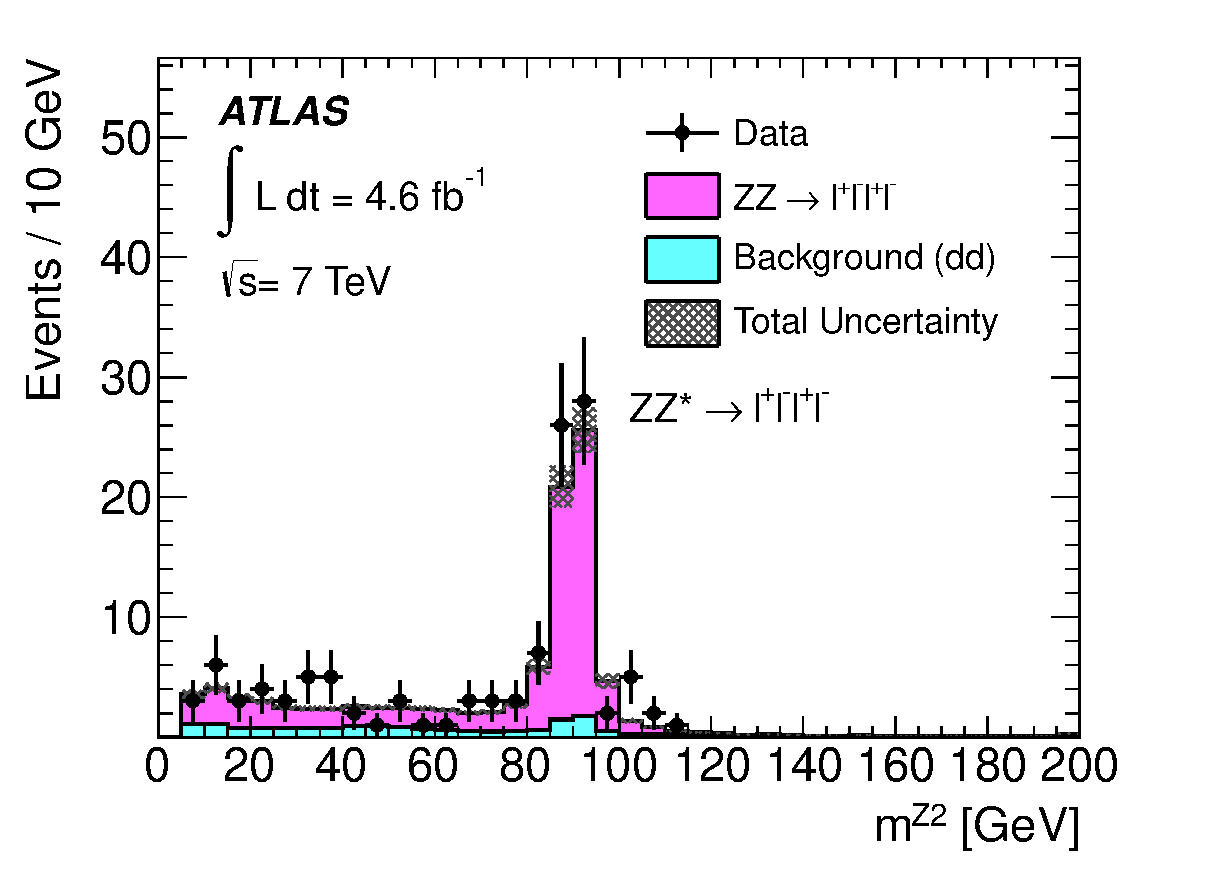
\includegraphics[width=0.47\textwidth]{7TeV/h_4l_ZZs_Z2_m}
     }
    \caption[Invariant masses of the (a) leading and (b) subleading \leppair\
    in candidate \ZZ\ events in the 7~\tev\ data.]
    {Invariant masses of the (a) leading and (b) subleading \leppair\ in
    candidate \ZZ\ events in the 7~\tev\ data. In each plot, the \leppair\
    not shown in the plot is required to pass the \sstooos\
    requirement. The points represent the observed data and the histograms show
    the prediction from simulation, where the background is normalised to the
    total background estimate as described in~\chap{BackgroundEstimate}.  The
    shaded band shows the combined statistical and systematic uncertainty on the
    prediction. 
}
    \label{fig:zzdists-Zmass-seven}
\end{center}
\end{figure}

% 8 TeV, Z1_m, Z2_m, m_Z>7GeV
\begin{figure}[htbp]
    \begin{center}
     \subfigure[]{
     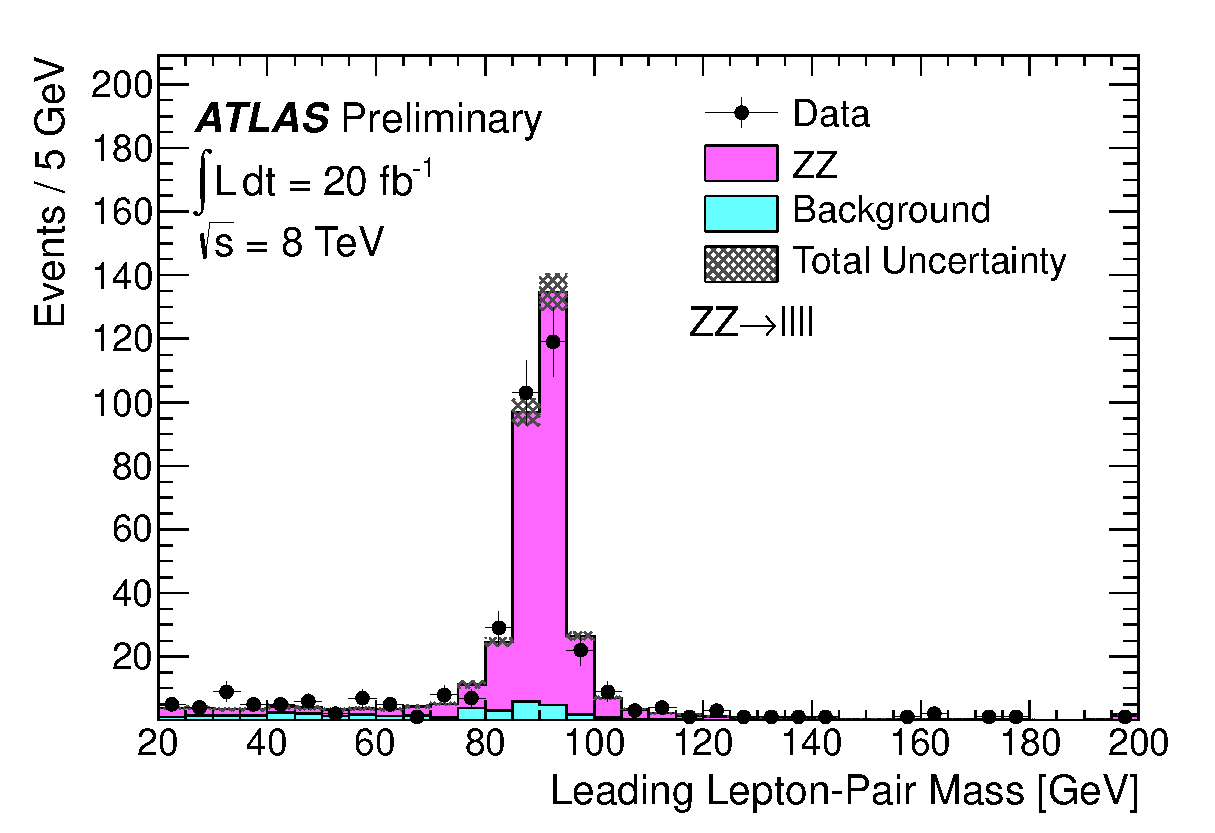
\includegraphics[width=0.47\textwidth]{8TeV/Z1_m_nm1_4l}
     }
     \subfigure[]{
     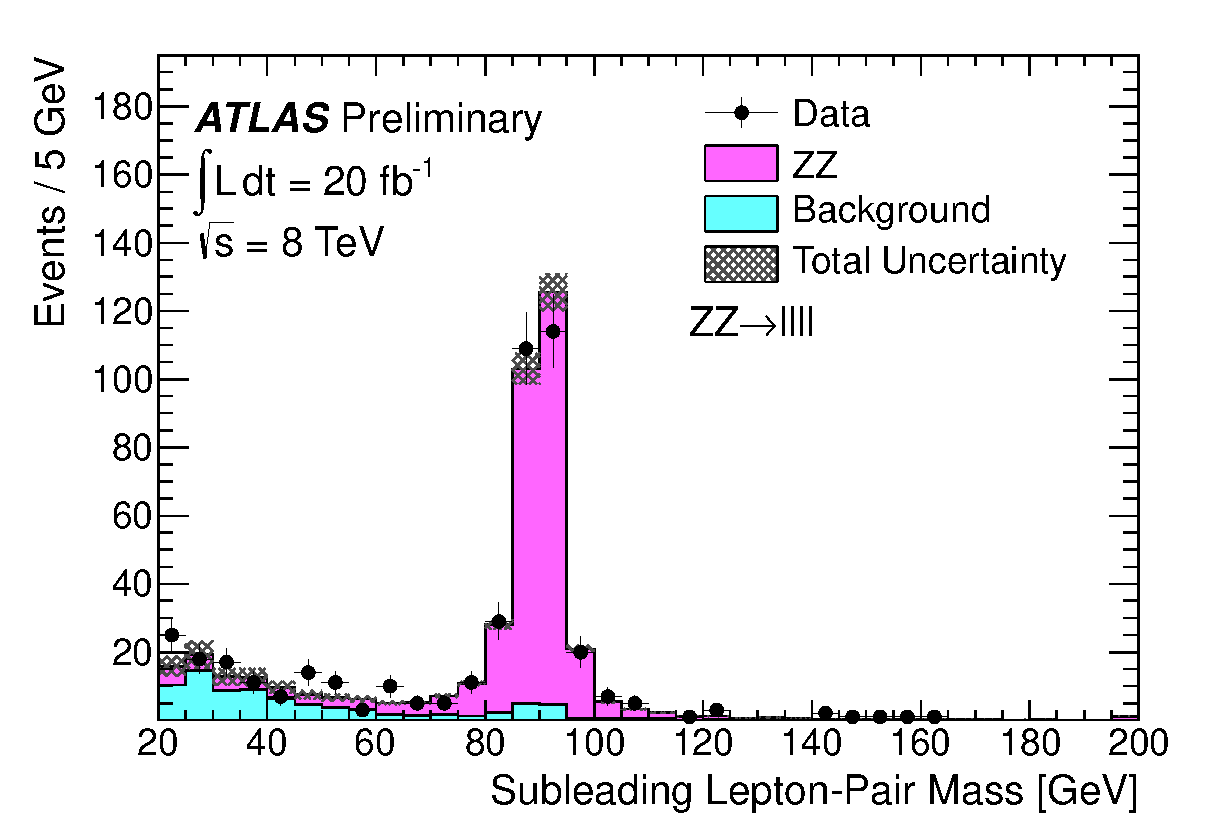
\includegraphics[width=0.47\textwidth]{8TeV/Z2_m_nm1_4l}
     }
    \caption[Invariant masses of the (a) leading and (b) subleading \leppair\
    in candidate \ZZ\ events in the 8~\tev\ data.]
    {Invariant masses of the (a) leading and (b) subleading \leppair\ in
    candidate \ZZ\ events in the 8~\tev\ data.  In each plot, the \leppair\    
    not shown in the plot is required to pass the \sstooos\
    requirement.  The points represent the observed data and the pink histogram
    shows the prediction for the signal from simulation. The light blue
    histogram shows the background shape obtained from data, normalised to the
    total background estimate as described in~\chap{BackgroundEstimate}.  The
    shaded band shows the combined statistical and systematic uncertainty on the
    prediction. 
}
    \label{fig:zzdists-Zmass-eight}
\end{center}
\end{figure}

% 7 TeV, ZZ, ZZ_pt / ZZ_m
\begin{figure}[htbp]
    \begin{center}
     \subfigure[]{
     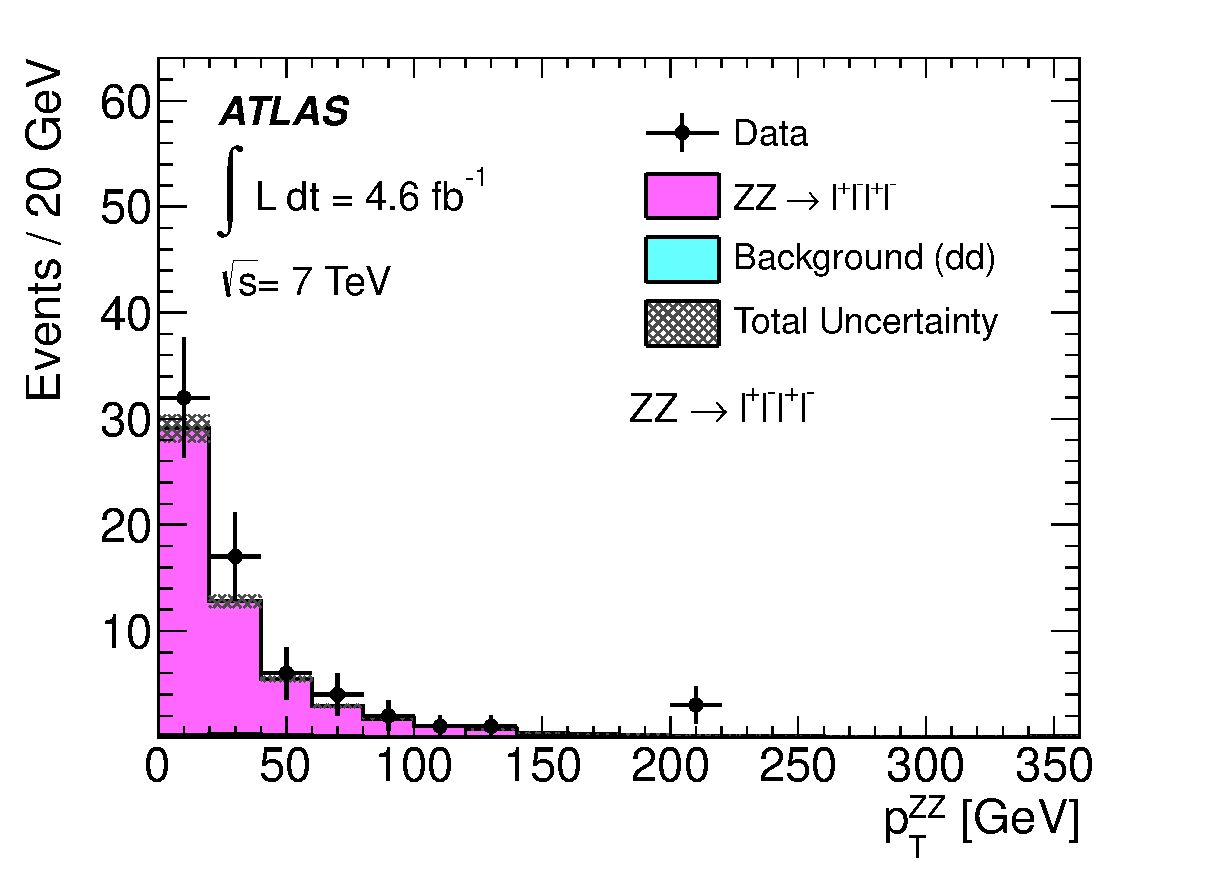
\includegraphics[width=0.47\textwidth]{7TeV/h_4l_ZZ_ZZ_pt}
     }
     \subfigure[]{
     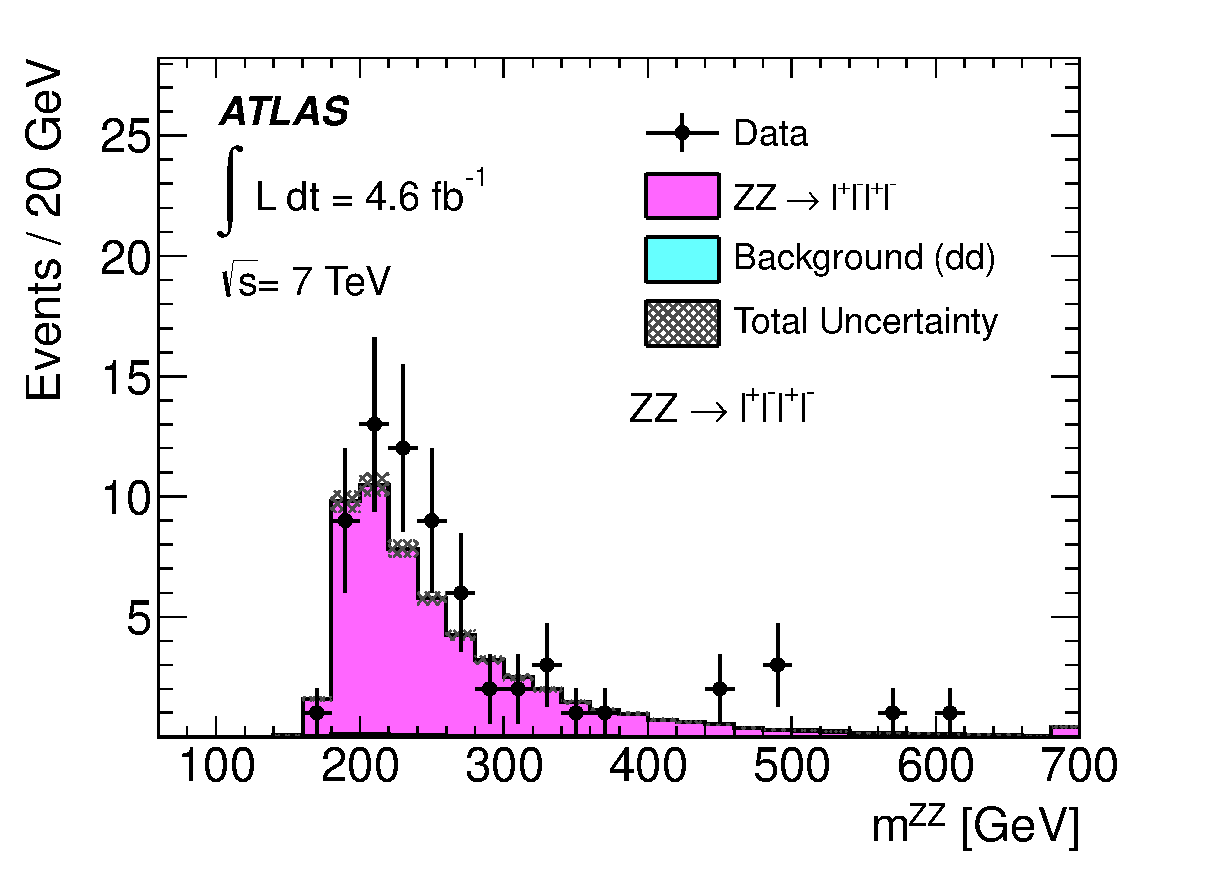
\includegraphics[width=0.47\textwidth]{7TeV/h_4l_ZZ_ZZ_m}
     }
     \subfigure[]{
     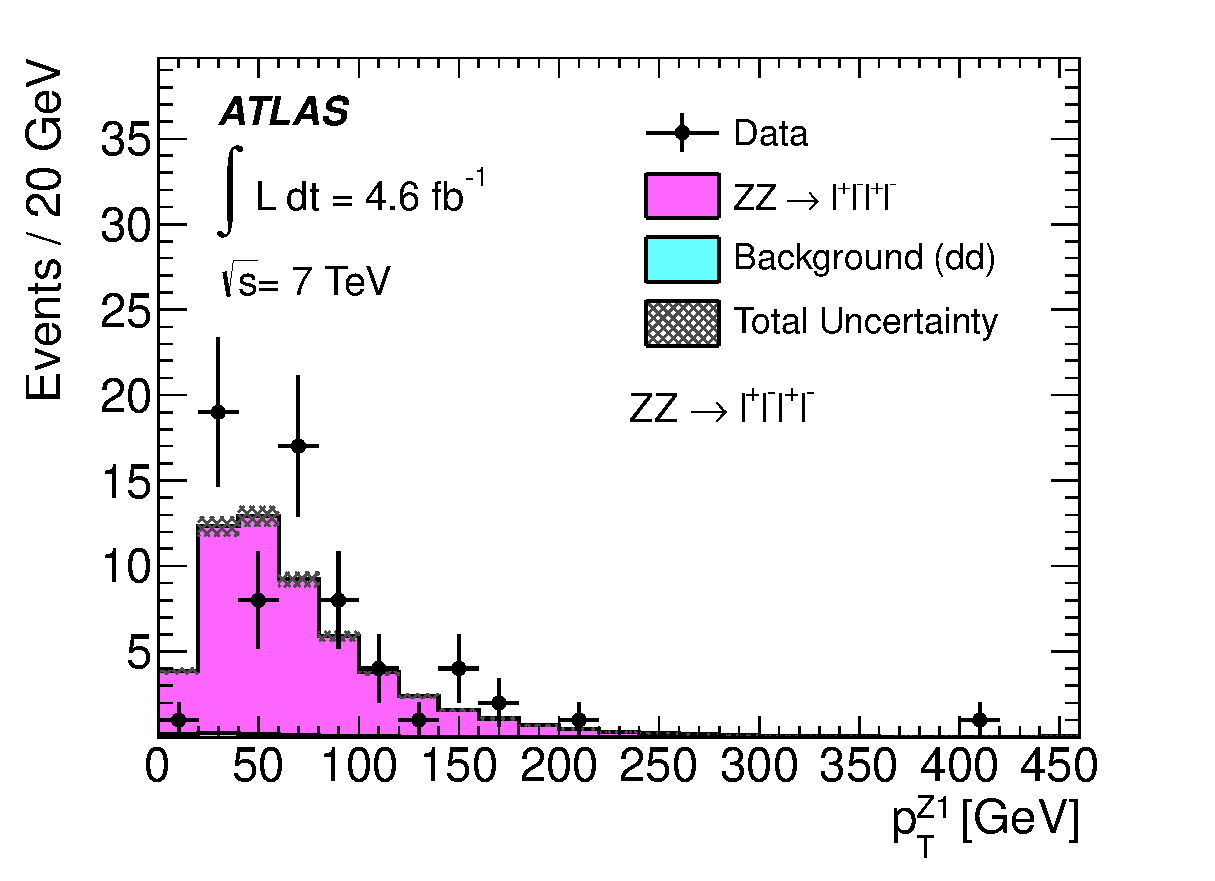
\includegraphics[width=0.47\textwidth]{7TeV/h_4l_ZZ_Z1_pt}
     }
     \subfigure[]{
     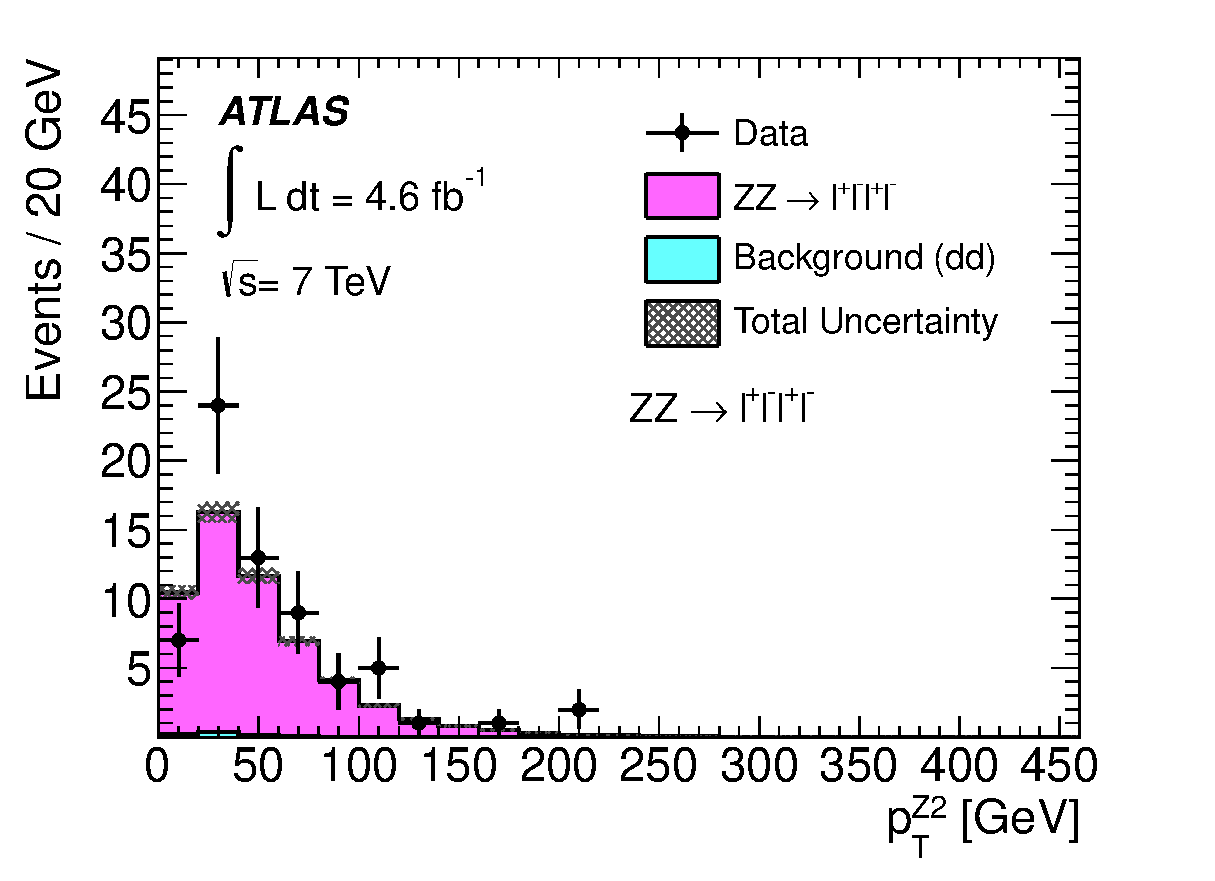
\includegraphics[width=0.47\textwidth]{7TeV/h_4l_ZZ_Z2_pt}
     }
    \caption[Kinematic distributions for events passing the \ZZ\ selection in
    the 7~\tev\ data.]
    {Kinematic distributions for events passing the \ZZ\ selection in
    the 7~\tev\ data: (a) transverse momentum $\pT^{\ZZ}$ and (b) invariant mass $m^{\ZZ}$ of the 
    four-lepton system, (c) transverse momentum of the leading
    \dilep\ pair $\pt^{Z1}$, and (d) transverse momentum of the subleading
    \dilep\ pair $\pt^{Z2}$. The points represent the observed data and the 
    histograms show the prediction from simulation, where the background
    is normalised to the total background estimate as described in
    ~\chap{BackgroundEstimate}. The shaded band 
    shows the combined statistical and systematic uncertainty on the prediction. 
    }
    \label{fig:zzdists-ZZ-seven}
    \end{center}
\end{figure}

% 8 TeV, ZZ, ZZ_pt / ZZ_m
\begin{figure}[htbp]
    \begin{center}
     \subfigure[]{
     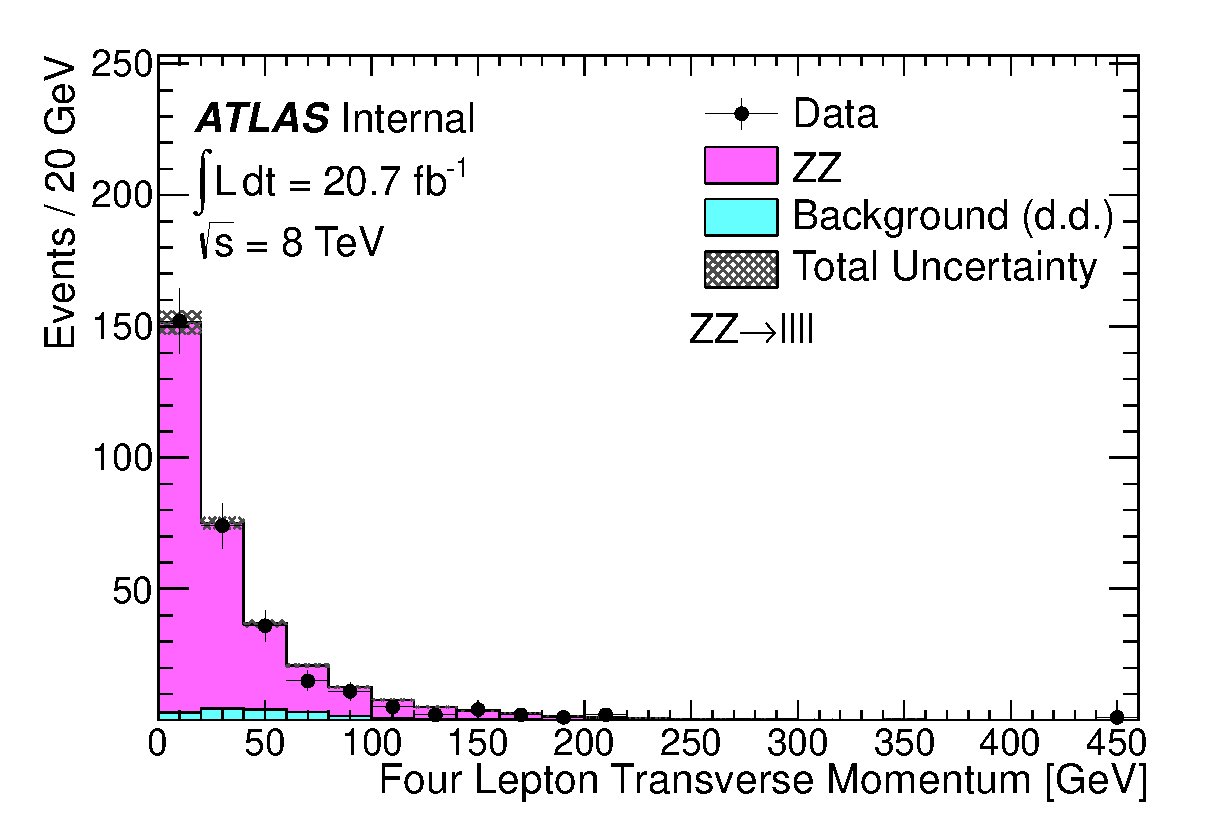
\includegraphics[width=0.47\textwidth]{8TeV/zzPt}
     }
     \subfigure[]{
     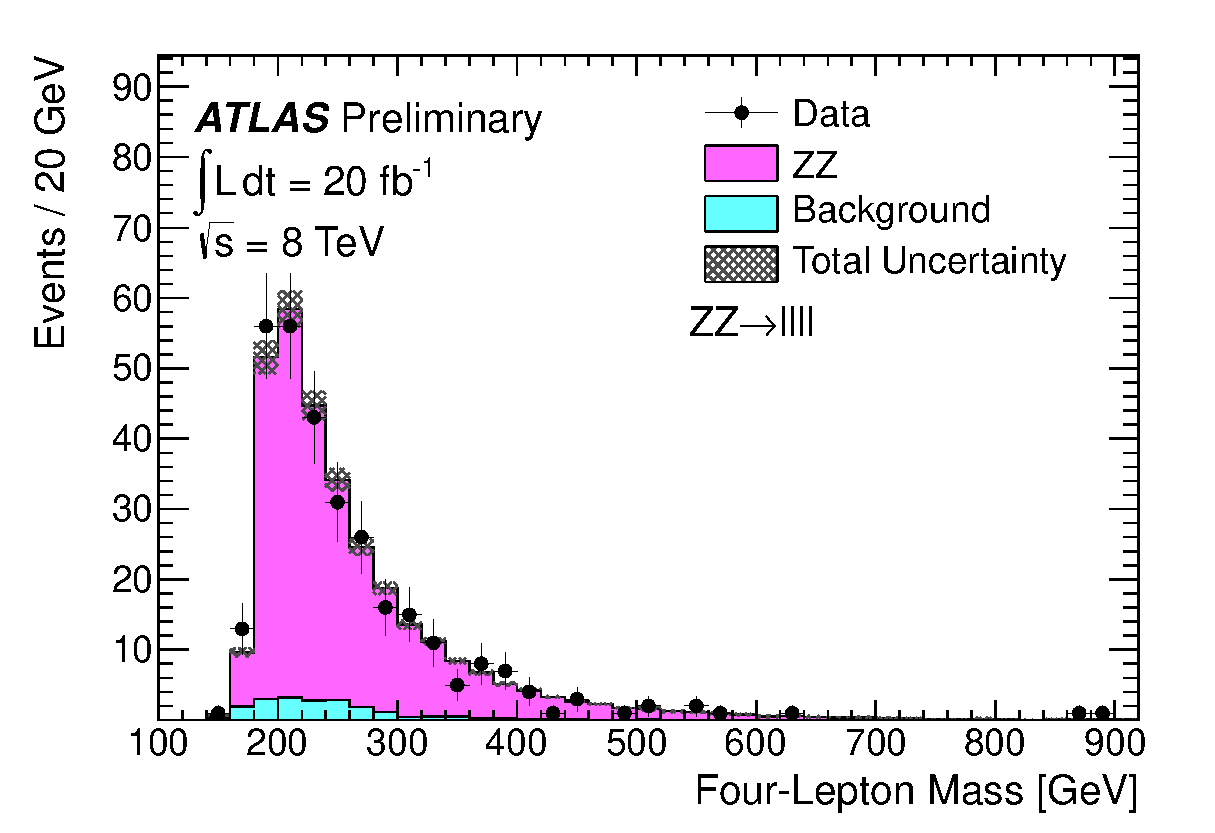
\includegraphics[width=0.47\textwidth]{8TeV/M4l}
     }
     \subfigure[]{
     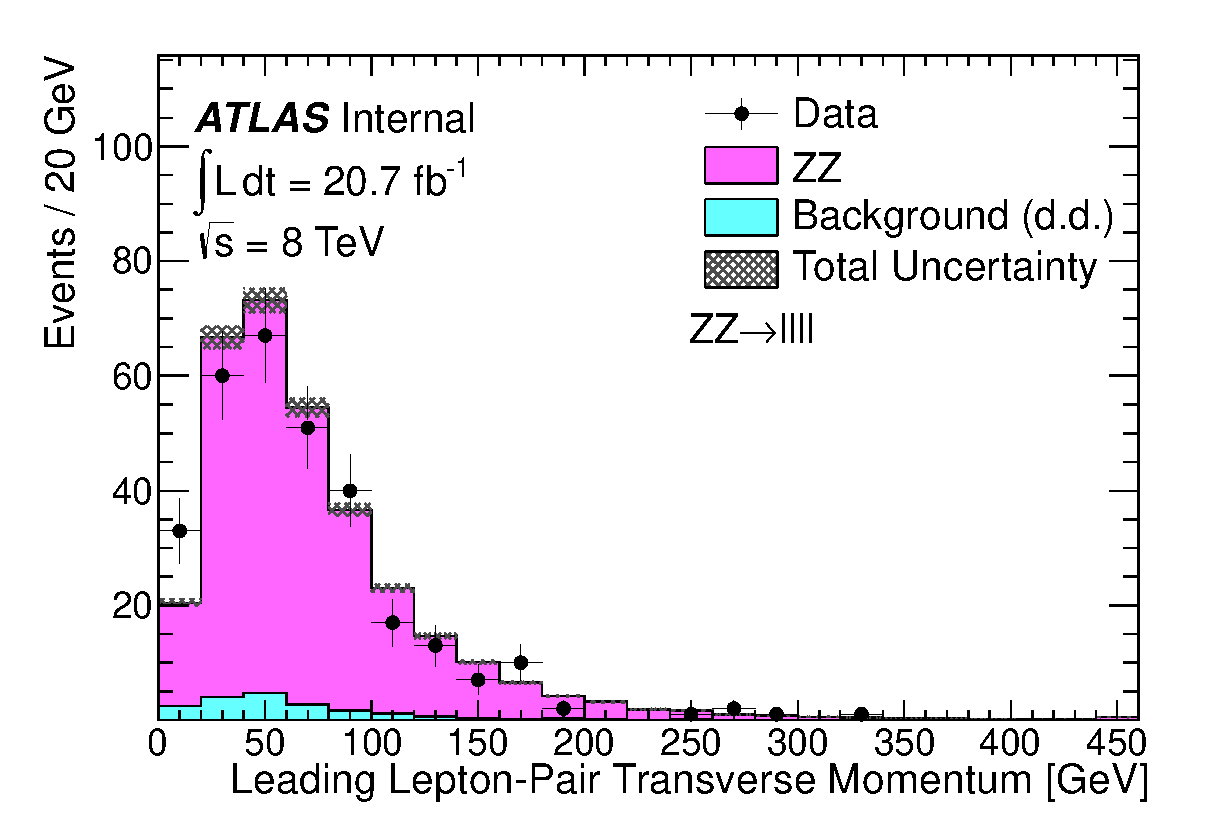
\includegraphics[width=0.47\textwidth]{8TeV/z1Pt}
     }
     \subfigure[]{
     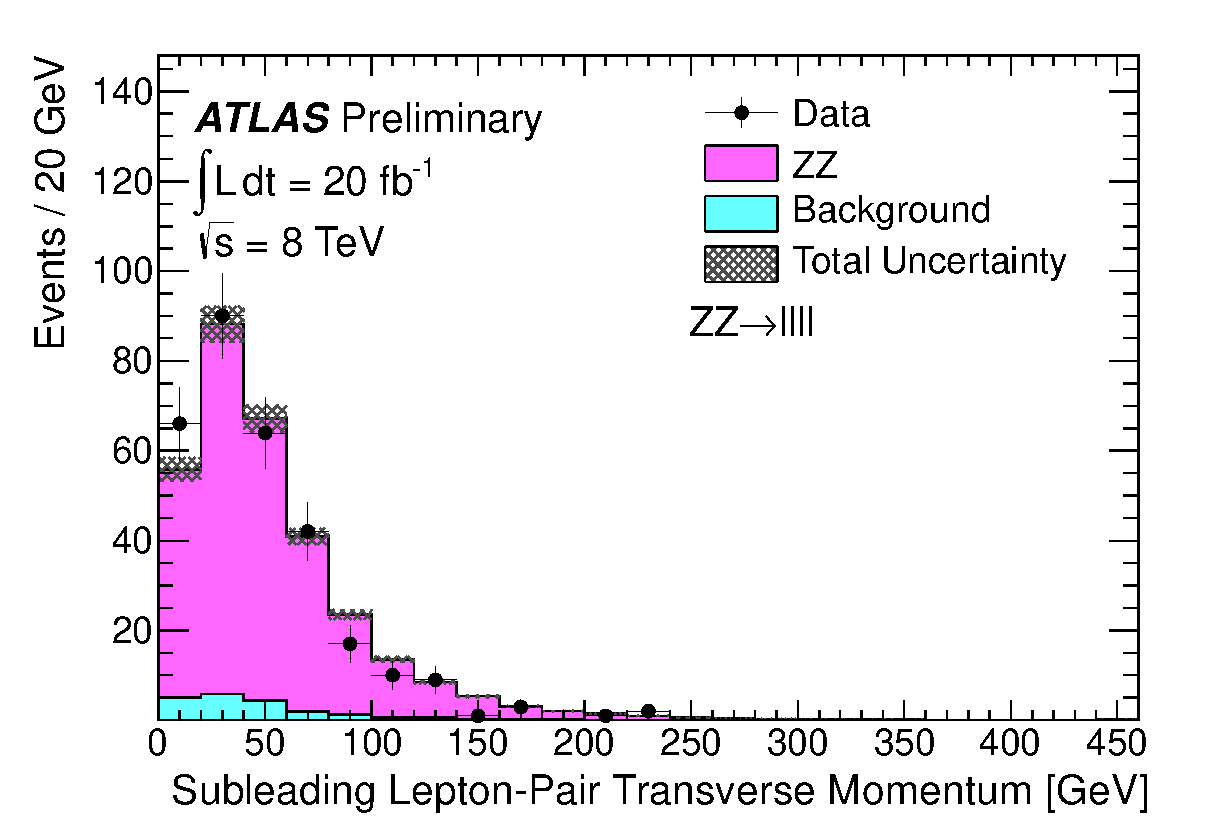
\includegraphics[width=0.47\textwidth]{8TeV/z2Pt}
     }
    \caption[Kinematic distributions for events passing the \ZZ\ selection in
    the 8~\tev\ data.]
    {Kinematic distributions for events passing the \ZZ\ selection in
    the 8~\tev\ data: (a) transverse momentum $\pT^{\ZZ}$ and (b) invariant mass $m^{\ZZ}$ of the 
    four-lepton system, (c) transverse momentum of the leading
    \dilep\ pair $\pt^{Z1}$, and (d) transverse momentum of the subleading
    \dilep\ pair $\pt^{Z2}$. The points represent the observed data and the pink histogram
    shows the prediction for the signal from simulation. The light blue
    histogram shows the background shape obtained from data, normalised to the
    total background estimate as described in~\chap{BackgroundEstimate}. The shaded band 
    shows the combined statistical and systematic uncertainty on the prediction. 
    }
    \label{fig:zzdists-ZZ-eight}
    \end{center}
\end{figure}
% 7 TeV, ZZ*, ZZ_pt / ZZ_m
\begin{figure}[htbp]
\begin{center}
    \subfigure[]{
    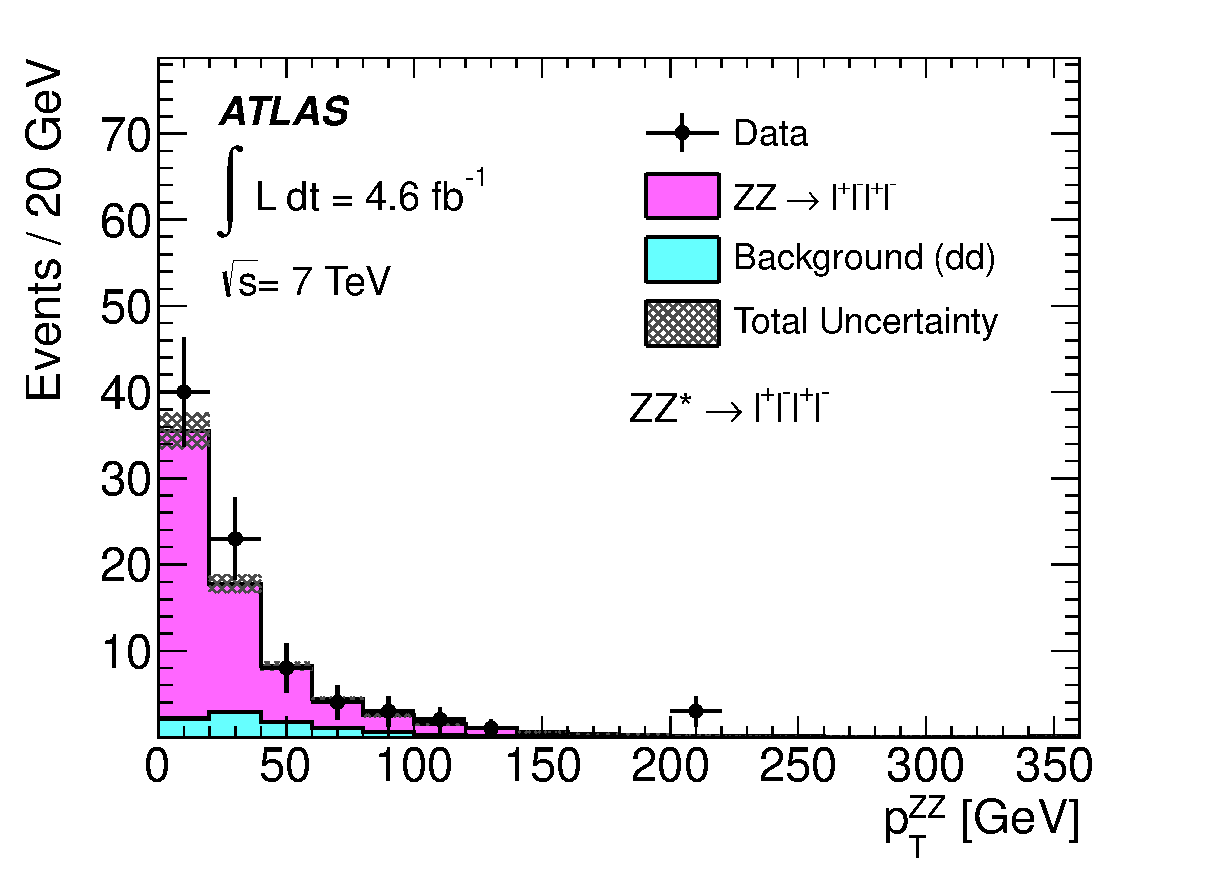
\includegraphics[width=0.47\textwidth]{7TeV/h_4l_ZZs_ZZ_pt}
    }
    \subfigure[]{
    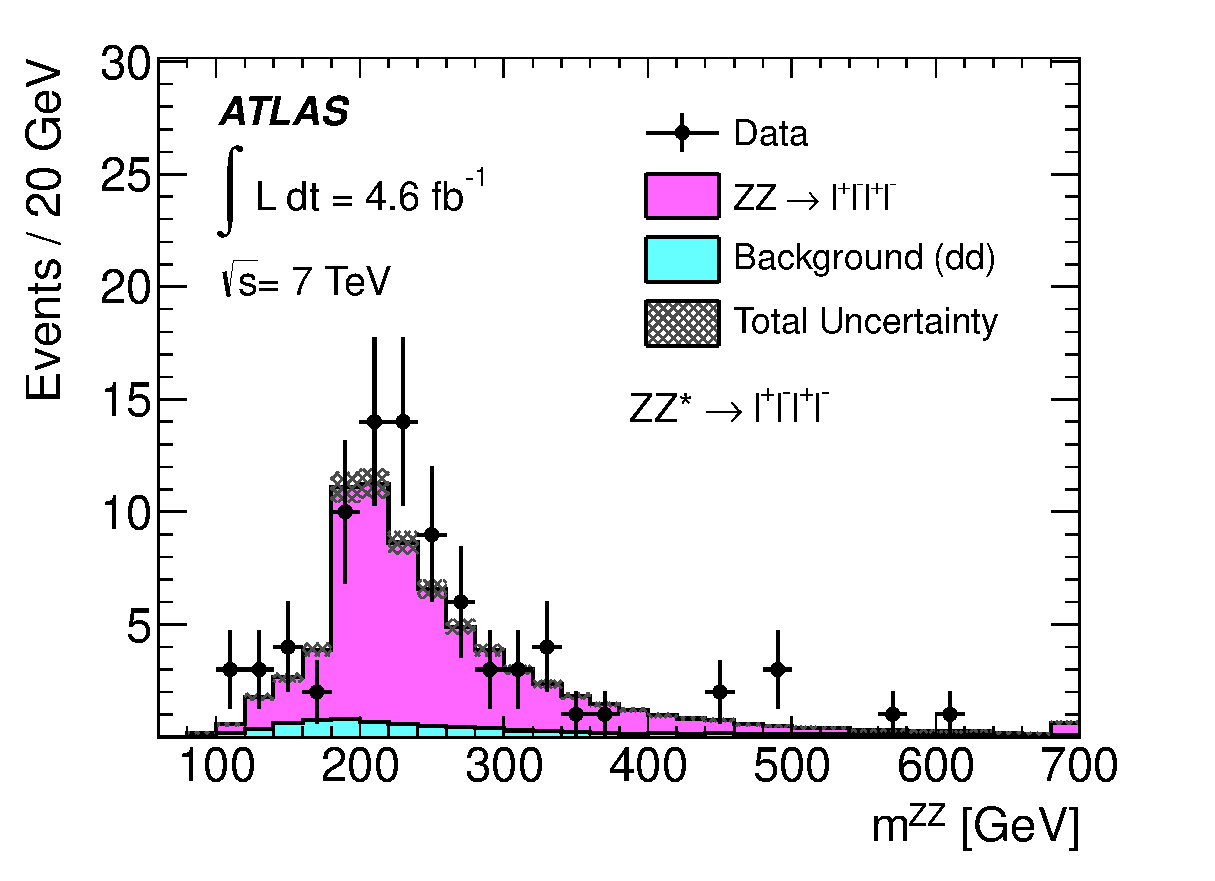
\includegraphics[width=0.47\textwidth]{7TeV/h_4l_ZZs_ZZ_m}
    }
    \subfigure[]{
    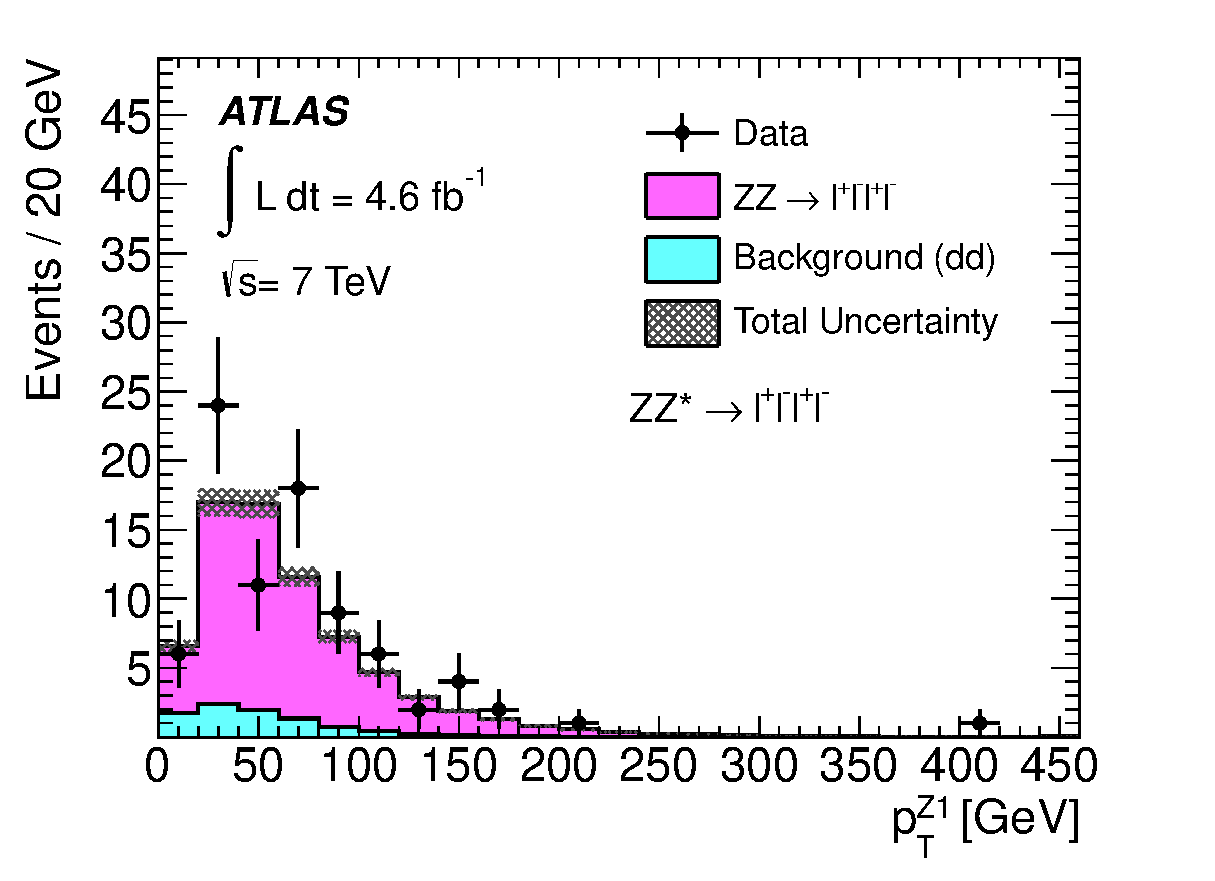
\includegraphics[width=0.47\textwidth]{7TeV/h_4l_ZZs_Z1_pt}
    }
    \subfigure[]{
    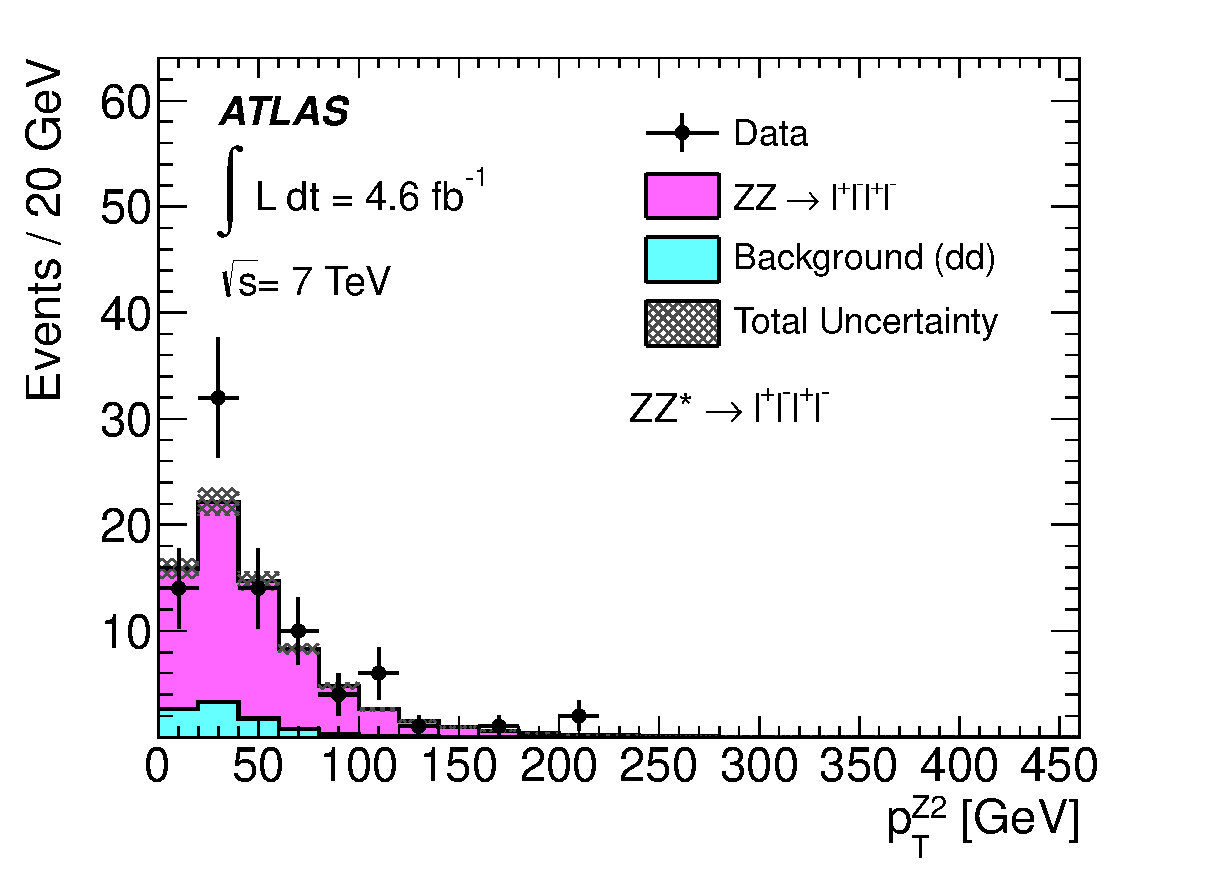
\includegraphics[width=0.47\textwidth]{7TeV/h_4l_ZZs_Z2_pt}
    }
    \caption[Kinematic distributions for events passing the \ZZs\ selection in
    the 7~\tev\ data.]
    {Kinematic distributions for events passing the \ZZs\ selection in
    the 7~\tev\ data: (a) transverse momentum $\pT^{\ZZ}$ and (b) invariant mass $m^{\ZZ}$ of the 
    four-lepton system, (c) transverse momentum of the leading
    \dilep\ pair $\pt^{Z1}$, and (d) transverse momentum of the subleading
    \dilep\ pair $\pt^{Z2}$. The points represent the observed data and the 
    histograms show the prediction from simulation, where the background
    is normalised to the data-driven estimate as described in
    ~\chap{BackgroundEstimate}. The shaded band 
    shows the combined statistical and systematic uncertainty on the prediction. 
    }
\end{center}
    \label{fig:zzdists-ZZs-seven}
\end{figure}


%% 8 TeV, ZZ*, ZZ_pt / ZZ_m
%\begin{figure}[htbp]
%\begin{center}
%    \subfigure[]{
%    
\includegraphics[width=0.47\textwidth]{placeholder}
%    }
%    \subfigure[]{
%    
\includegraphics[width=0.47\textwidth]{placeholder}
%    }
%    \subfigure[]{
%    
\includegraphics[width=0.47\textwidth]{placeholder}
%    }
%    \subfigure[]{
%    
\includegraphics[width=0.47\textwidth]{placeholder}
%    }
%    \caption[Kinematic distributions for events passing the \ZZs\ selection in
%    the 8~\tev\ data.]
%    {Kinematic distributions for events passing the \ZZs\ selection in
%    the 8~\tev\ data: (a) transverse momentum $\pT^{\ZZ}$ and (b) invariant mass $m^{\ZZ}$ of the 
%    four-lepton system, (c) transverse momentum of the leading
%    \dilep\ pair $\pt^{Z1}$, and (d) transverse momentum of the subleading
%    \dilep\ pair $\pt^{Z2}$. The points represent the observed data and the 
%    histograms show the prediction from simulation, where the background
%    is normalised to the data-driven (dd) estimate as described in
%    ~\chap{BackgroundEstimate}. The shaded band 
%    shows the combined statistical and systematic uncertainty on the prediction. 
%    }
%\end{center}
%    \label{fig:zzdists-ZZs-eight}
%\end{figure}

\section{\CX\ Measurement}

As discussed in~\sec{TheoryZZProduction-CxDef}, the \cx\ is first measured in a fiducial phase-space
corresponding to the experimental selections (the \intro{fiducial \cx}), in
order to reduce systematic uncertainties associated with the extrapolation. The
fiducial \cx\ is then extrapolated to the total \ZZ\ \cx, correcting for the
acceptance of the fiducial phase-space and the \ZZllll\ branching fraction.  The definition of the
fiducial phase-space was given in~\sec{TheoryZZProduction-CxDef}, and is slightly different for the
7~\tev\ and 8~\tev\ analyses due to the differing experimental selections.

\subsection{Fiducial \CX}

For a given \ZZllll\ final state the fiducial cross section is defined as:

\begin{equation}\label{eq:xsecfid_fourl}
\sigmaFidZZlllplp = \frac{\NObslllplp - \NBglllplp}{\mathcal{L} \times \CZZ^{\lllplp}}
\end{equation}
where \NObs\ and \NBg\ are the number of observed events and the expected number
of background events, respectively, $\mathcal{L}$ is the integrated luminosity
of the data samples and
$\CZZ^{\lllplp}$ is the reconstruction acceptance factor for the \lllplp\
final-state, as defined in~\sec{objSel-CZZ}.

The \cx\ is estimated using a maximum profile likelihood technique, by
maximising the \intro{profile likelihood function, \L} with respect to the \cx.
\L\ is the product of the Poisson probability ($P$) for observing $N$ events given a
\cx\ $\sigma$, reconstruction acceptance \CZZ\ and background $b$; and Gaussian
distributions (G) to describe nuisance parameters due to uncertainties on \CZZ\
and on $b$:

\begin{equation}
\small
   \L(\sigma, \CZZ', b'; \Delta_{b}, \Delta_{C_{ZZ}}, N) = P(\sigma, \CZZ^\prime,
   b^\prime; N)\times G(\CZZ^\prime; C_{ZZ}, \Delta_{C_{ZZ}}) \times G(b^\prime; b, \Delta_{b})
\end{equation}

The Poisson probability to observe $N$ events given an expected
number of signal events $s$ and expected background $b$ is:

\begin{equation}
P(\sigma, C_{ZZ}, b; N) =
\frac{e^{-(s+b)}\cdot
     \left(s+b\right)^{N}}
     {N!},
\end{equation}
where $s=s(\sigmaFid, \CZZ)$ is given by:

\begin{equation}
   s(\sigmaFid, \CZZ) = \sigmaFid\times\mathcal{L}\times\CZZ \\
\end{equation}

In practice, for computational convenience $-\ln(L)$ is minimised rather
than maximising $L$, however the procedures are equivalent. The fiducial
\cx\ for each final-state is calculated separately. For calculating the combined \ZZllll\
fiducial \cx, the number of observed and expect events for each individual
final-state are summed and the weighted average of the reconstruction
acceptances in each final-state is taken. A combined background estimate is used,
estimating the background for all \llll\ final states together; this benifits from a
lower statistical uncertainty than simply summing the individual final-state background
estimates. This procedure for combining the final-states gives the highest weight to the highest
statistics channels, and does not automatically take into account the better
signal over background ratios ($S/B$) in different final-states. However, since the
lowest statistics channel is also the channel with the worse $S/B$ (the \eeee\
final-state), this simpler approach is justified.

\subsubsection{Fiducial \CX\ Results}

Fiducial \cx\ results are presented in~\tab{meas-fid-cx}. {\bf Some comment here
on agreement with theory and comparison 7~\tev\ and 8~\tev}.

%% Observed Fiducial Cross Sections, 7 TeV
\begin{table}
\renewcommand\arraystretch{1.3}
\centering
\small
  \begin{tabular}{lll}
    \hline\hline
     Channel & Measured Fiducial \CX   & Theory                              \\
     %7~\tev, \ZZ             &                          \\
    \hline
     {\bf \underline{7~\tev, \ZZ}}             &                          \\
     \ZZeeee\       & \ZZSevenTeVFiducialCrossSectionZZEEEE   & \ZZSevenTeVTheoryFiducialCrossSectionZZEEEE \\
     \ZZmmmm\       & \ZZSevenTeVFiducialCrossSectionZZMMMM   & \ZZSevenTeVTheoryFiducialCrossSectionZZMMMM \\
     \ZZeemm\       & \ZZSevenTeVFiducialCrossSectionZZEEMM   & \ZZSevenTeVTheoryFiducialCrossSectionZZEEMM \\
     \ZZllll\   & \ZZSevenTeVFiducialCrossSectionZZLLLL   & \ZZSevenTeVTheoryFiducialCrossSectionZZLLLL \\
    %\hline\hline
    %\\
    %\hline\hline
     %7~\tev, \ZZs             &                          \\
    \hline
     {\bf \underline{7~\tev, \ZZs}}             &                          \\
     \ZZseeee\      & \ZZSevenTeVFiducialCrossSectionZZsEEEE & \ZZSevenTeVTheoryFiducialCrossSectionZZsEEEE   \\
     \ZZsmmmm\      & \ZZSevenTeVFiducialCrossSectionZZsMMMM & \ZZSevenTeVTheoryFiducialCrossSectionZZsMMMM   \\
     \ZZseemm\      & \ZZSevenTeVFiducialCrossSectionZZsEEMM & \ZZSevenTeVTheoryFiducialCrossSectionZZsEEMM   \\
     \ZZsllll\  & \ZZSevenTeVFiducialCrossSectionZZsLLLL & \ZZSevenTeVTheoryFiducialCrossSectionZZsLLLL   \\
    \hline
     {\bf \underline{8~\tev, \ZZ}}             &                          \\
     \ZZeeee\       & \ZZSevenTeVFiducialCrossSectionZZEEEE & \ZZEightTeVTheoryFiducialCrossSectionZZEEEE   \\
     \ZZmmmm\       & \ZZSevenTeVFiducialCrossSectionZZMMMM & \ZZEightTeVTheoryFiducialCrossSectionZZMMMM   \\
     \ZZeemm\       & \ZZSevenTeVFiducialCrossSectionZZEEMM & \ZZEightTeVTheoryFiducialCrossSectionZZEEMM   \\
     \ZZllll\   & \ZZSevenTeVFiducialCrossSectionZZLLLL & \ZZEightTeVTheoryFiducialCrossSectionZZLLLL   \\
    %\hline\hline
    %\\
    %\hline\hline
     %7~\tev, \ZZs             &                          \\
    \hline
     {\bf \underline{8~\tev, \ZZs}}             &                          \\
     \ZZseeee\      & \ZZSevenTeVFiducialCrossSectionZZsEEEE & \ZZEightTeVTheoryFiducialCrossSectionZZsEEEE   \\
     \ZZsmmmm\      & \ZZSevenTeVFiducialCrossSectionZZsMMMM & \ZZEightTeVTheoryFiducialCrossSectionZZsMMMM   \\
     \ZZseemm\      & \ZZSevenTeVFiducialCrossSectionZZsEEMM & \ZZEightTeVTheoryFiducialCrossSectionZZsEEMM   \\
     \ZZsllll\  & \ZZSevenTeVFiducialCrossSectionZZsLLLL & \ZZEightTeVTheoryFiducialCrossSectionZZsLLLL   \\
    \hline\hline
  \end{tabular}

      \caption[Fiducial \CX\ measurements at 7~\tev\ and at 8~\tev.]
      { Fiducial \CX\ measurements at 7~\tev\ and at 8~\tev. The second column
      gives the measured \cx, and the third the prediction from theory,
      calculated using MCFM with PDF set CT10 and scale set to
      $\frac{1}{2}m(\ZZ)$. } 
    \label{table:meas-fid-cx}
\renewcommand\arraystretch{1}
\end{table}

    %\calc{1+2}

\subsection{Total \CX}

The total cross-section is obtained by extrapolating the fiducial \cx\ from the
fiducial phase-space to the total phase space and by correcting for the \ZZllll\
branching fraction. The total \cx\ is defined with both \Z\ bosons with mass
\sstooosZ. In order to extrapolate from the fiducial to the total-phase
space the \intro{fiducial acceptance factor}, \AZZ\ must be estimated. \AZZ\ is
the is fraction of \ZZ\ events with both \Z\ bosons in the \sstooosZ\ mass range which fall into the fiducial phase-space, and is
estimated from \mcsim\ as:

\begin{equation}
\AZZ = \frac{ N^{\rm MC\ Fiducial\ Volume}_{{\rm Generated}\ ZZ} }{ N^{{\rm MC\
All}}_{{\rm Generated}\ ZZ} }
\end{equation}
The total \cx\ is then defined as:

\begin{equation}\label{eq:xsectot_fourl}
\sigmaTotZZ = \frac{ \NObs - \NBg}{\mathcal{L} \times
BR\{\ZZllll\} \times \AZZ \times \CZZ}
\end{equation}
Uncertainties on \AZZ\ arise due to uncertainties on the \partDF, the choice of
the factorisation and renormalisation scales and modelling of the parton shower
and ISR. \AZZ\ is determined using the \powhegbox\ and \ggtwoZZ\ generators. The
PDF errors are estimated using the 52 CT10 error sets and by taking the
difference with MSTW2008, and the scale errors are estimated by varying the scales
up and down by a factor of two. The systematic due to the modelling of the parton shower
and ISR is estimated by comparing the value for \AZZ\ obtained from a
\powhegbox\ sample showered with \herwig\ compared to to the nominal sample
which is showered with \pythia. Additionally, the difference with the \AZZ\
obtained from MCFM, which does not model the parton shower, is taken as an
additional systematic. The contributions of these different sources of
systematic uncertainty are shown in~\tab{azz-syst}, and the values of \AZZ\ are
shown in~\tab{azz}.
% 1.1 % quoted in note seems to be difference between having showering and not,
% ie MCFM vs Powheg

\begin{table}
\renewcommand\arraystretch{1.1}
\centering
\small
  \begin{tabular}{lll}
    \hline\hline
     Source (\%) & 7~\tev & 8~\tev \\
    \hline
     PDF  & \ZZSevenTeVAZZPDFUncPercentage\ & \ZZEightTeVAZZPDFUncPercentage \\
     Scale  & \ZZSevenTeVAZZScaleUncPercentage\ & \ZZEightTeVAZZScaleUncPercentage \\
     Parton Shower / ISR Model  & \ZZSevenTeVAZZISRUncPercentage\ & \ZZEightTeVAZZISRUncPercentage \\
     Generator Difference  & \ZZSevenTeVAZZGenUncPercentage\ & \ZZEightTeVAZZGenUncPercentage \\
     \hline
     Total  & \ZZSevenTeVAZZTotalUncPercentage\ & \ZZEightTeVAZZTotalUncPercentage \\
    \hline\hline
  \end{tabular}

      \caption[Systematic uncertainties to the fiducial acceptance factors, \AZZ, at 7~\tev\ and at 8~\tev.]
      { Systematic uncertainties to the fiducial acceptance factors, \AZZ, at
      7~\tev\ and at 8~\tev. }
    \label{table:azz-syst}
\renewcommand\arraystretch{1}
\end{table}


\begin{table}
\renewcommand\arraystretch{1.1}
\centering
\small
  \begin{tabular}{lll}
    \hline\hline
     Channel & 7~\tev & 8~\tev \\
    \hline
     \ZZeeee\       &
     \measSyst{\ZZSevenTeVAZZCentral}{\errSym{\ZZSevenTeVAZZSystUnc}}   & 
     \measSyst{\ZZEightTeVAZZCentral}{\errSym{\ZZEightTeVAZZSystUnc}}   \\
     \ZZmmmm\       &
     \measSyst{\ZZSevenTeVAZZCentral}{\errSym{\ZZSevenTeVAZZSystUnc}}   & 
     \measSyst{\ZZEightTeVAZZCentral}{\errSym{\ZZEightTeVAZZSystUnc}}   \\
     \ZZeemm\       &
     \measSyst{\ZZSevenTeVAZZCentral}{\errSym{\ZZSevenTeVAZZSystUnc}}   & 
     \measSyst{\ZZEightTeVAZZCentral}{\errSym{\ZZEightTeVAZZSystUnc}}   \\
     \ZZllll\       &
     \measSyst{\ZZSevenTeVAZZCentral}{\errSym{\ZZSevenTeVAZZSystUnc}}   & 
     \measSyst{\ZZEightTeVAZZCentral}{\errSym{\ZZEightTeVAZZSystUnc}}   \\
    \hline\hline
  \end{tabular}

      \caption[Fiducial acceptance factors, \AZZ, at 7~\tev\ and at 8~\tev.]
      { Fiducial acceptance factors, \AZZ, at 7~\tev\ and at 8~\tev. Systematic
      uncertainties are shown; the statistical uncertainty is negligable.} 
    \label{table:azz}
\renewcommand\arraystretch{1}
\end{table}


\subsubsection{Total \CX\ Results}

Total \cx\ results are presented in~\tab{meas-tot-cx}. {\bf Some comment here
on agreement with theory and comparison 7~\tev\ and 8~\tev}.

%% Observed Total Cross Sections
\begin{table}
\renewcommand\arraystretch{1.8}
\centering
\small
  \begin{tabular}{lll}
    \hline\hline
     & Measured \CX   & Theory                              \\
     %7~\tev, \ZZ             &                          \\
    \hline
     %{\bf \underline{7~\tev}}             &                          \\
     \sigmaTotZZ(\sqrtseq{7})\   & \ZZSevenTeVTotalCrossSection & \ZZSevenTeVTheoryTotalCrossSection \\
    %\hline
     %{\bf \underline{8 \ZZ}}             &                          \\
     \sigmaTotZZ(\sqrtseq{8})\   & \ZZEightTeVTotalCrossSection & \ZZEightTeVTheoryTotalCrossSection \\
    \hline\hline
  \end{tabular}

      \caption[Total \ZZ\ \CX\ measurements at 7~\tev\ and at 8~\tev.]
      { Total \ZZ\ \CX\ measurements at 7~\tev\ and at 8~\tev. The second column
      gives the measured \cx, and the third the prediction from theory,
      calculated using MCFM with PDF set CT10 and scale set to
      $\frac{1}{2}m(\ZZ)$. } 
    \label{table:meas-tot-cx}
\renewcommand\arraystretch{1}
\end{table}


\section{Unfolded Kinematic Distributions}

The observed kinematic distributions shown in Figures~\ref{fig:zzdists-ZZ-seven}
to~\ref{fig:zzdists-ZZ-eight} are a convolution of the underlying `true'
distribution of the parameter of interest and a distortion and smearing due to
detector effects. Although 
%for the expected \ZZ\ signal distribution shown in
%these figures 
the detector distortion is included in the \mc\ simulation shown in those
figures, allowing a comparison of the
theoretical prediction and the observed data, it is desirable to correct the
observed distributions for detector effects in order to allow model independent
comparisons between theory and observation and to allow comparison between
different experiments. The correction procedure is referred
to as \intro{unfolding}. 

Formally, one can consider some parameter of interest $x$,
distributed according to a probability distribution function (\probDF) $f(x)$. Due to experimental effects, one
does not measure $x$ but a different variable $y$, distributed
according to a different \probDF\ $g(y)$. The measured variable $y$ is related to $x$ by a
convolution of the true distribution $f(x)$ with some response function to account for the
experimental effects $A(y,x)$:
\begin{equation}
\int A(y,x)f(x){\rm d}x = g(y)
\label{eqn:unfold-conv}
\end{equation}

In practice, continuous distributions are generally not measured, but instead
measurements are made
in discretised bins. $x$ and $y$ can thus be rewritten as
vectors \unfx\ and \unfy, where each element represents the number of events in
a given bin. The response
function then becomes a response matrix \unfA, ~\eqn{unfold-conv} can be
rewritten as:
\begin{equation}
\mathbf{Ax} = \mathbf{y}
\label{eqn:unfold-conv-matrix}
\end{equation}

An iterative Bayesian algorithm~\cite{2010arXiv1010.0632D} is used to perform
the unfolding, 
using the implementation provided by the {\sc
RooUnfold}~\cite{2011arXiv1105.1160A} package. The algorithm treats the response
matrix \unfA\ as a description of the probability of observing some particular data given the
true distribution. From Bayes's theorem, the probability of there being 
\unfxi\ events in bin $i$ of the true distribution arising due to
\unfyj\ events in bin $j$ is given by:
\begin{equation}
P(\unfxi|\unfyj,I) = \frac{P(\unfyj|\unfxi,I)\cdot P(\unfxi|I)}{\sum_{k}P(\unfyk|\unfxk,I)\cdot P(\unfxk|I)}
\end{equation}
where $I$ represents the state of information under which the analysis is
performed, and $P(\unfxi|I)$ is the prior for \unfxi. $P(\unfyi|\unfxj,I)$ can
be associated with element $ij$ of the unfolding matrix \unfA. This
probability can be used to `share' the observed events between the bins of the
true distribution. The estimate of the true spectrum is occurred by repeating
this `sharing' for all the bins of the observed distribution and taking into
account the efficiency. The estimate for the number of counts in bin $i$ of the
true distribution \unfxi\ is thus given by:
\begin{equation}
\unfxi = \frac{1}{\epsilon_{i}} \sum^{n}_{j=1} \frac{A_{ji} \cdot P(\unfxi|I)}{\sum_k A_{jk} \cdot P(\unfxk|I)}
\end{equation}
where $\epsilon_{i}=\Sigma^{n}_{j} A_{j}$ accounts for the efficiency.

It takes as an initial prior for \unfx\ the simulated distribution from
\mc\ and iterates, taking the posterior distribution from one iteration as a
prior for the next. The choice of initial prior will tend to bias the unfolded
distribution, but this bias decreases steeply with the number of iterations. The
statistical uncertainty tends to increase with the number of iterations, as
fluctuations can be amplified by positive feedback inherent in the algorithm;
the number of iterations must thus be chosen to balance the bias due to the
choice of prior and amplification of statistical uncertainties. It is found that
the difference in the results between three and four iterations is much smaller than
the statistical uncertainty. The results for three iterations are thus taken as
the nominal result, and the difference between three and four iterations is
taken as an additional systematic. 

Statistical uncertainties due to the number of observed events are assessed by
pseudo-experiments, in each experiment fluctuating the observed \unfy\ by a
Poisson distribution and re-running the full unfolding procedure; the RMS of 2000
pseudo-experiments is taken as the statistical uncertainty. 
The response matrix \unfA\ is estimated from \mc\ simulation and
will thus have associated systematic uncertainties due to experimental
uncertainties. These are handled in a similar manner to the statistical
uncertainties, re-running the unfolding procedure multiple times and varying the
\unfA\ according to the different sources of systematic uncertainty. An
additional systematic arises from the choice of prior. This is estimated by
using the distribution predicted by \sherpa\ as a prior instead of the nominal
\powhegbox. 

Distributions of three variables sensitive to new phenomena are selected for
unfolding: the transverse momentum \ptZ\ of the leading \Z\ boson candidate, the
angle \deltaPhiLL\ between the decay leptons
of the leading \Z\ boson candidate, and the four-lepton invariant mass \mZZ. Bin
boundaries are chosen to maximise sensitivity to nTGCs, and are in all cases
larger than the detector resolution. The unfolded distributions are presented in
terms of a differential fiducial \cx, and are shown
in~\fig{unfolded-distributions} (unfolded distributions are only provided for
the 7~\tev\ analysis). The \sm\ prediction is consistent with the
measurement in each case. The uncertainty on the unfolded distributions is dominated by the
statistical uncertainty, which is approximately 30\% in most bins. The
systematic uncertainty is no more than 5\% in each bin, and is dominated by the
uncertainty arising due to the choice of prior.

\begin{figure}[htbp]
\begin{center}
\subfigure[]{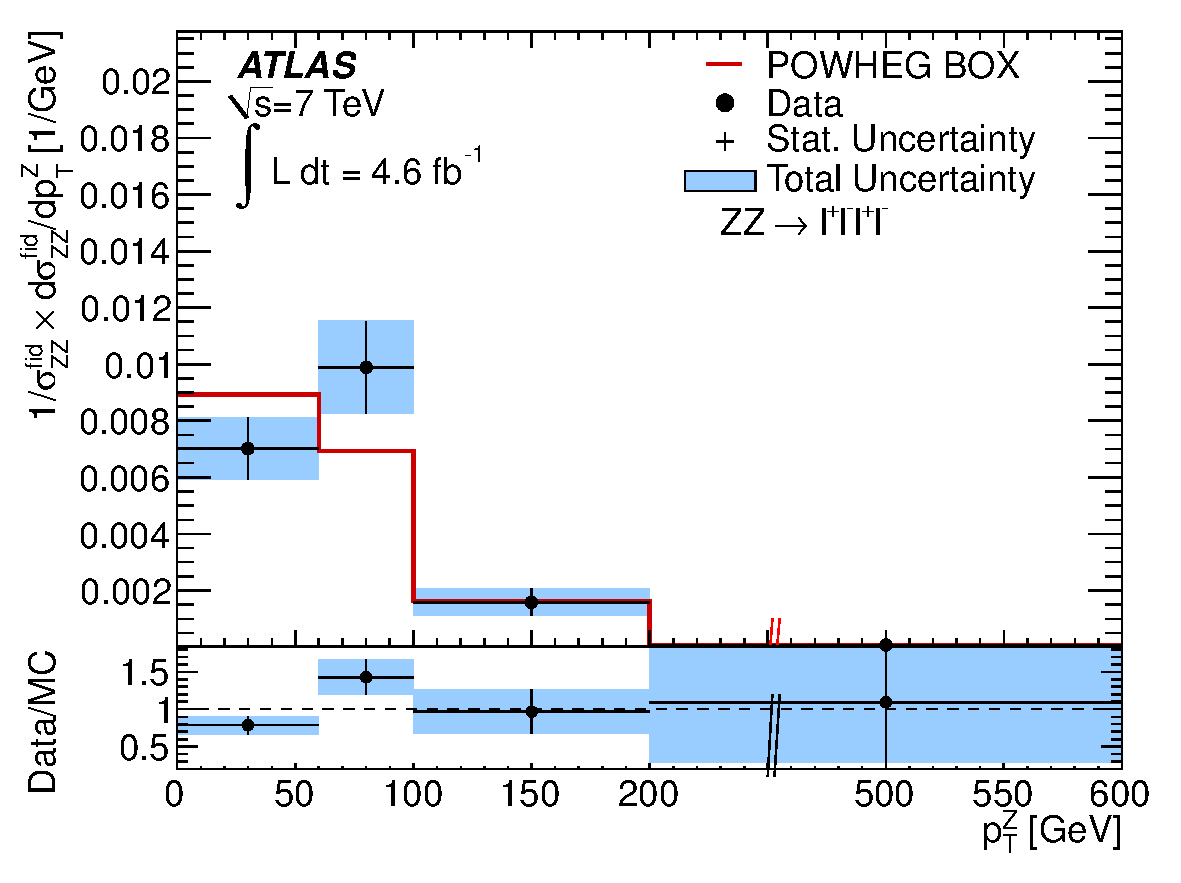
\includegraphics[width=0.57\textwidth]{Unfolded/ZZllll_ZpT_natbins_UnfoldedDistribution}}
\subfigure[]{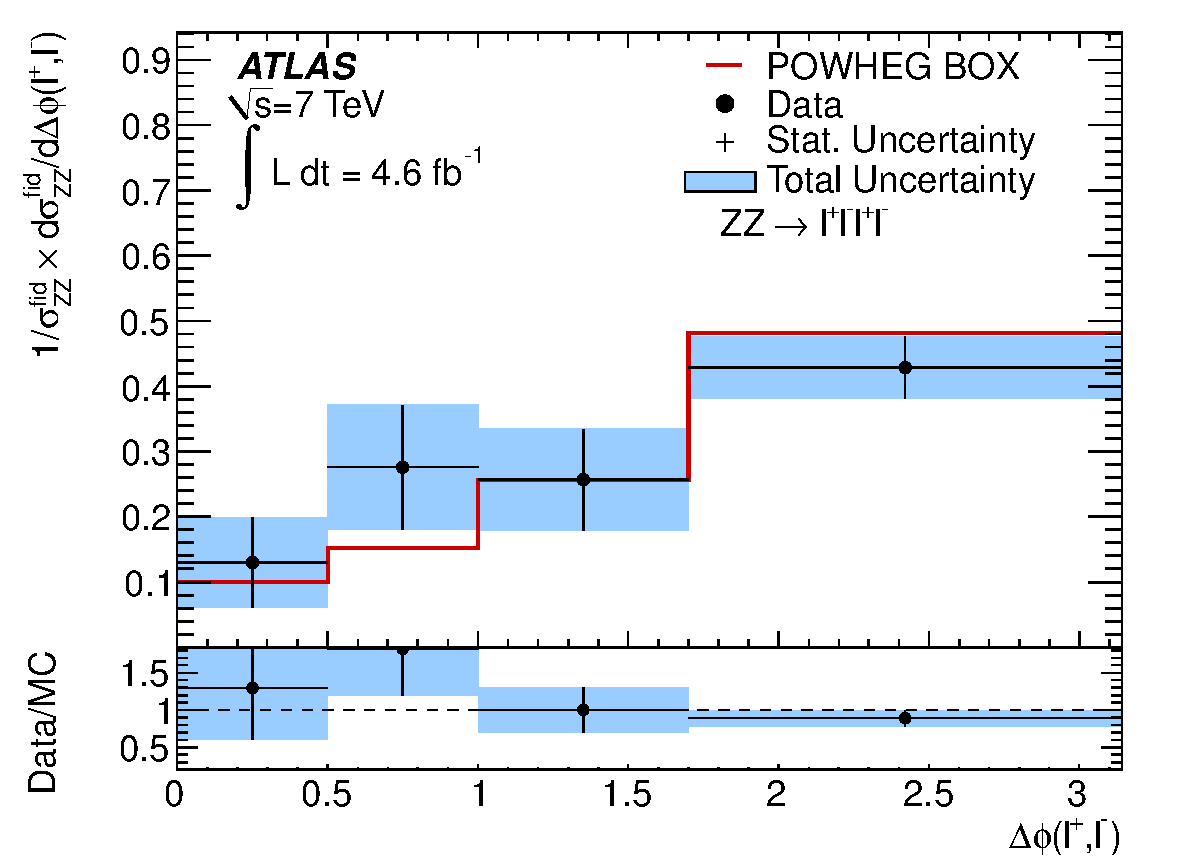
\includegraphics[width=0.57\textwidth]{Unfolded/ZZllll_DPhiLep_natbins_UnfoldedDistribution}}
\subfigure[]{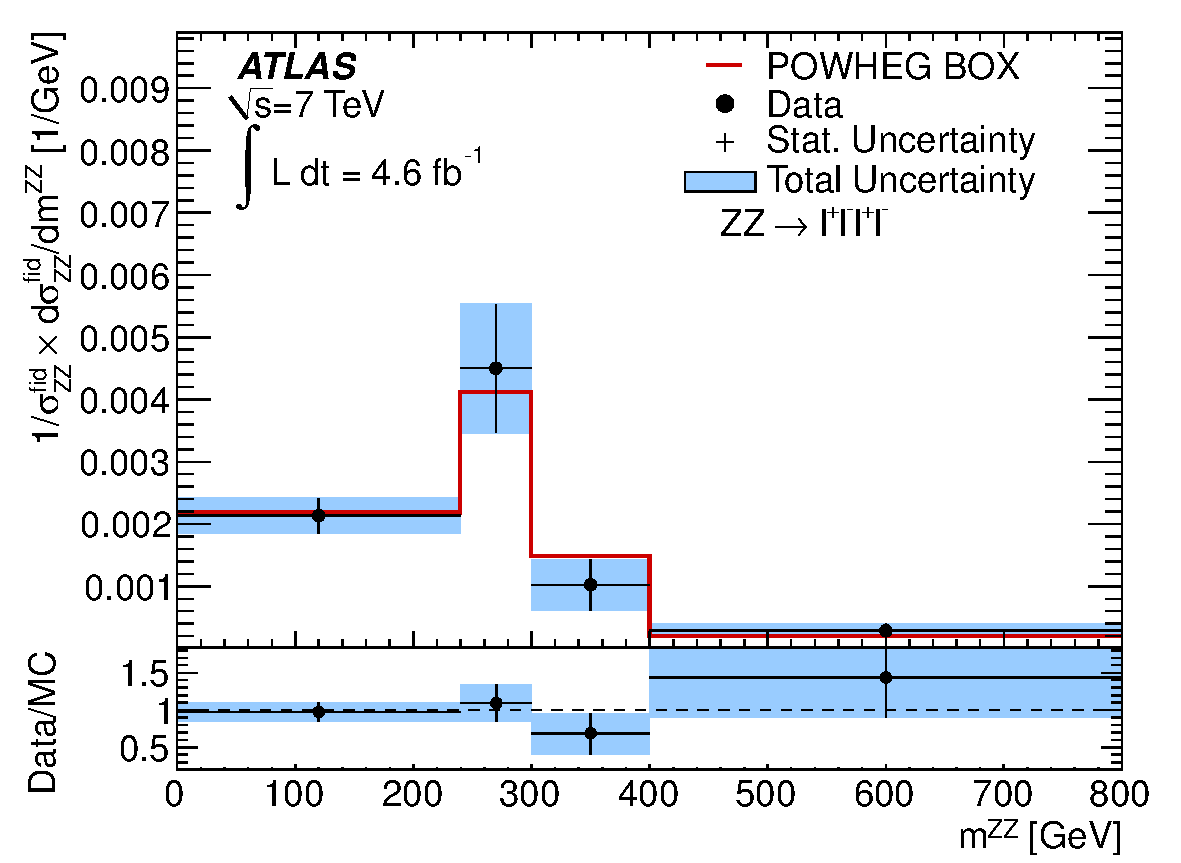
\includegraphics[width=0.57\textwidth]{Unfolded/ZZllll_ZZTMass_natbins_UnfoldedDistribution}}
\caption{\label{fig:unfolded-distributions}Unfolded \ZZ\ fiducial \cx s
in bins of (a) the
\pT\ of the leading \Z\ boson, (b) the angle between the decay leptons
of the leading \Z\ boson, \deltaPhiLL\ and (c) the four-lepton invariant mass,
\mZZ. }
\end{center}
\end{figure}

